% This is the Reed College LaTeX thesis template. Most of the work
% template. Later comments etc. by Ben Salzberg (BTS). Additional
% restructuring and APA support by Jess Youngberg (JY).
% Your comments and suggestions are more than welcome; please email
% them to cus@reed.edu
%
% See http://web.reed.edu/cis/help/latex.html for help. There are a
% great bunch of help pages there, with notes on
% getting started, bibtex, etc. Go there and read it if you're not
% already familiar with LaTeX.
%
% Any line that starts with a percent symbol is a comment.
% They won't show up in the document, and are useful for notes
% to yourself and explaining commands.
% Commenting also removes a line from the document;
% very handy for troubleshooting problems. -BTS

% As far as I know, this follows the requirements laid out in
% the 2002-2003 Senior Handbook. Ask a librarian to check the
% document before binding. -SN

%%
%% Preamble
%%
% \documentclass{<something>} must begin each LaTeX document
\documentclass[12pt,twoside]{reedthesis}
% Packages are extensions to the basic LaTeX functions. Whatever you
% want to typeset, there is probably a package out there for it.
% Chemistry (chemtex), screenplays, you name it.
% Check out CTAN to see: http://www.ctan.org/
%%
\usepackage{graphicx,latexsym}
\usepackage{amsmath}
\usepackage{amssymb,amsthm}
\usepackage{longtable,booktabs,setspace}
\usepackage{chemarr} %% Useful for one reaction arrow, useless if you're not a chem major
\usepackage{rotating}

% Modified by CII
\usepackage[hyphens]{url}
\usepackage{hyperref}
\usepackage{lmodern}

% Added by CII (Thanks, Hadley!)
% Use ref for internal links
\renewcommand{\hyperref}[2][???]{\autoref{#1}}
\def\chapterautorefname{Chapter}
\def\sectionautorefname{Section}
\def\subsectionautorefname{Subsection}

\usepackage{caption}
\captionsetup{width=5in}

% \usepackage{times} % other fonts are available like times, bookman, charter, palatino

\title{Consumption and Cooptation of Care: a statistical analysis of visits to
urgent care}
\author{Kaitlyn R. Jackson}
% The month and year that you submit your FINAL draft TO THE LIBRARY (May or December)
\date{May 2016}
\division{History and Social Sciences}
\advisor{Jessica Epstein}
%If you have two advisors for some reason, you can use the following
\altadvisor{}
%%% Remember to use the correct department!
\department{Sociology}
% if you're writing a thesis in an interdisciplinary major,
% uncomment the line below and change the text as appropriate.
% check the Senior Handbook if unsure.
%\thedivisionof{The Established Interdisciplinary Committee for}
% if you want the approval page to say "Approved for the Committee",
% uncomment the next line
%\approvedforthe{Committee}

% Below added by CII

%%% Copied from knitr
%% maxwidth is the original width if it's less than linewidth
%% otherwise use linewidth (to make sure the graphics do not exceed the margin)
\makeatletter
\def\maxwidth{ %
  \ifdim\Gin@nat@width>\linewidth
    \linewidth
  \else
    \Gin@nat@width
  \fi
}
\makeatother

\renewcommand{\contentsname}{Table of Contents}

\setlength{\parskip}{0pt}


\providecommand{\tightlist}{%
  \setlength{\itemsep}{0pt}\setlength{\parskip}{0pt}}

\Acknowledgements{
I want to thank a few people, mostly my mom. Will fill in when this is
dOnE.
}

\Dedication{
Right now? to coffee
}

\Preface{

}

\Abstract{
Urgent care centers are a relatively new and emergent phenomemnon in the
American health care system, yet little to no academic reasearch has
been performed on how they are situated in the larger sociological
understanding of the healthcare system. This thesis attempts to further
such an understanding by examining the typologies of patients which are
the users of urgent care, and further, who of those uses such centers as
their primary care physicians.
}

\usepackage{tikz} \usepackage{setspace} \usepackage{amsmath}
\usepackage{natbib} \usepackage{rotating} \usepackage{longtable}
\pagestyle{plain}

%%
%% End Preamble
%%
%

\begin{document}

      \maketitle
  
  \frontmatter % this stuff will be roman-numbered
  \pagestyle{empty} % this removes page numbers from the frontmatter

      \begin{acknowledgements}
      I want to thank a few people, mostly my mom. Will fill in when this is
      dOnE.
    \end{acknowledgements}
  
  
  % Add table of abbreviations?

      \hypersetup{linkcolor=black}
    \setcounter{tocdepth}{2}
    \tableofcontents
  
      \listoftables
  
      \listoffigures
  
      \begin{abstract}
      Urgent care centers are a relatively new and emergent phenomemnon in the
      American health care system, yet little to no academic reasearch has
      been performed on how they are situated in the larger sociological
      understanding of the healthcare system. This thesis attempts to further
      such an understanding by examining the typologies of patients which are
      the users of urgent care, and further, who of those uses such centers as
      their primary care physicians.
    \end{abstract}
  
      \begin{dedication}
      Right now? to coffee
    \end{dedication}
  
  \mainmatter % here the regular arabic numbering starts
  \pagestyle{fancyplain} % turns page numbering back on

  \chapter*{Introduction}\label{introduction}
  \addcontentsline{toc}{chapter}{Introduction}
  
  \setcounter{chapter}{1} \setcounter{section}{0} \doublespacing
  
  The days of having a local doctor who cared for all of a patient's
  health needs are long gone. In their place, a rapidly expanding and
  complex network of healthcare providers and services have developed,
  increasingly placing the burden on the patient to make the appropriate
  choice. In particular, the past twenty years have seen a surge in a new
  type of medical practice known as urgent care centers, and the industry
  shows no sign of slowing down. Yet given such rapid expansion of the
  industry, it is surprising that little academic research has taken
  urgent care as its subject. In part a response to this oversight, the
  following analysis will use a representative sample of urgent care
  center visits to examine the use patterns of these facilities in recent
  years. I investigate three central questions regarding urgent care: what
  are the typologies of patients using urgent care, how can we use this
  information to situate urgent care centers into the larger complex of
  the American healthcare system, and what does the sociological research
  offer to an understanding of this relatively new phenomenon?
  
  There is no official definition of what constitutes an urgent care
  center, but the scope of services provided generally falls between that
  of a primary care doctor's office and an emergency department. The
  centers typically focus on acute episodic care, and have a substantial
  emphasis on customer service. Most are open past the hours of a
  traditional primary care practice, and often have a wider variety of
  services, such as labs, x-rays and other emergency department equipment
  (Weinick and Betancourt n.d.).
  
  While the industry is currently experiencing rapid growth, the concept
  got off to a rocky start. The first urgent care centers opened in the
  United States in the early 1980's., with no more than a handful in
  operation at the time. Unfortunately, (at least as far as early
  investors were concerned), the industry rapidly declined, and the few
  clinics which had opened were largely absorbed into larger hospitals and
  healthcare groups. Ten years later, in the mid-1990's , the centers
  began expanding rapidly, growing to over 12,000 centers today. By the
  UCAOA's estimate, in 2014, approximately two new urgent care centers
  were opening in the United States each week (Becker n.d.).
  
  Such recent and rapid expansion has been heavily examined by the media,
  which often attribute growth to a diverse set of market factors such as
  long wait times for primary care appointments, crowded emergency
  departments and patient demand for more accessible care, including
  after-hours appointments (Yee, Lechner, and Boukus 2013). Yet despite
  the rapid development of the industry and the great interest
  sociologists have historically taken in America's health care system,
  hardly any scholarly research has been done on why these centers are
  coming to play a major part of the healthcare system or what their
  patterns of use are. While many are quick to point towards long wait
  times, and the difficulty of finding doctors in the current healthcare
  system, the repercussions of the new turn towards urgent care centers
  are not well known, nor has their place in the American healthcare
  system been examined.
  
  \section{National Trends in the Urgent Care
  Industry}\label{national-trends-in-the-urgent-care-industry}
  
  Most urgent care centers operate in metro areas, though they are not
  restricted to cities. The services offered are compared with hospital
  emergency departments and traditional primary clare clinics in table 1
  below, which was presented in the official state of California industry
  overview of urgent care compiled in 2011. \newpage
  
  \begin{figure}[htbp]
  \centering
  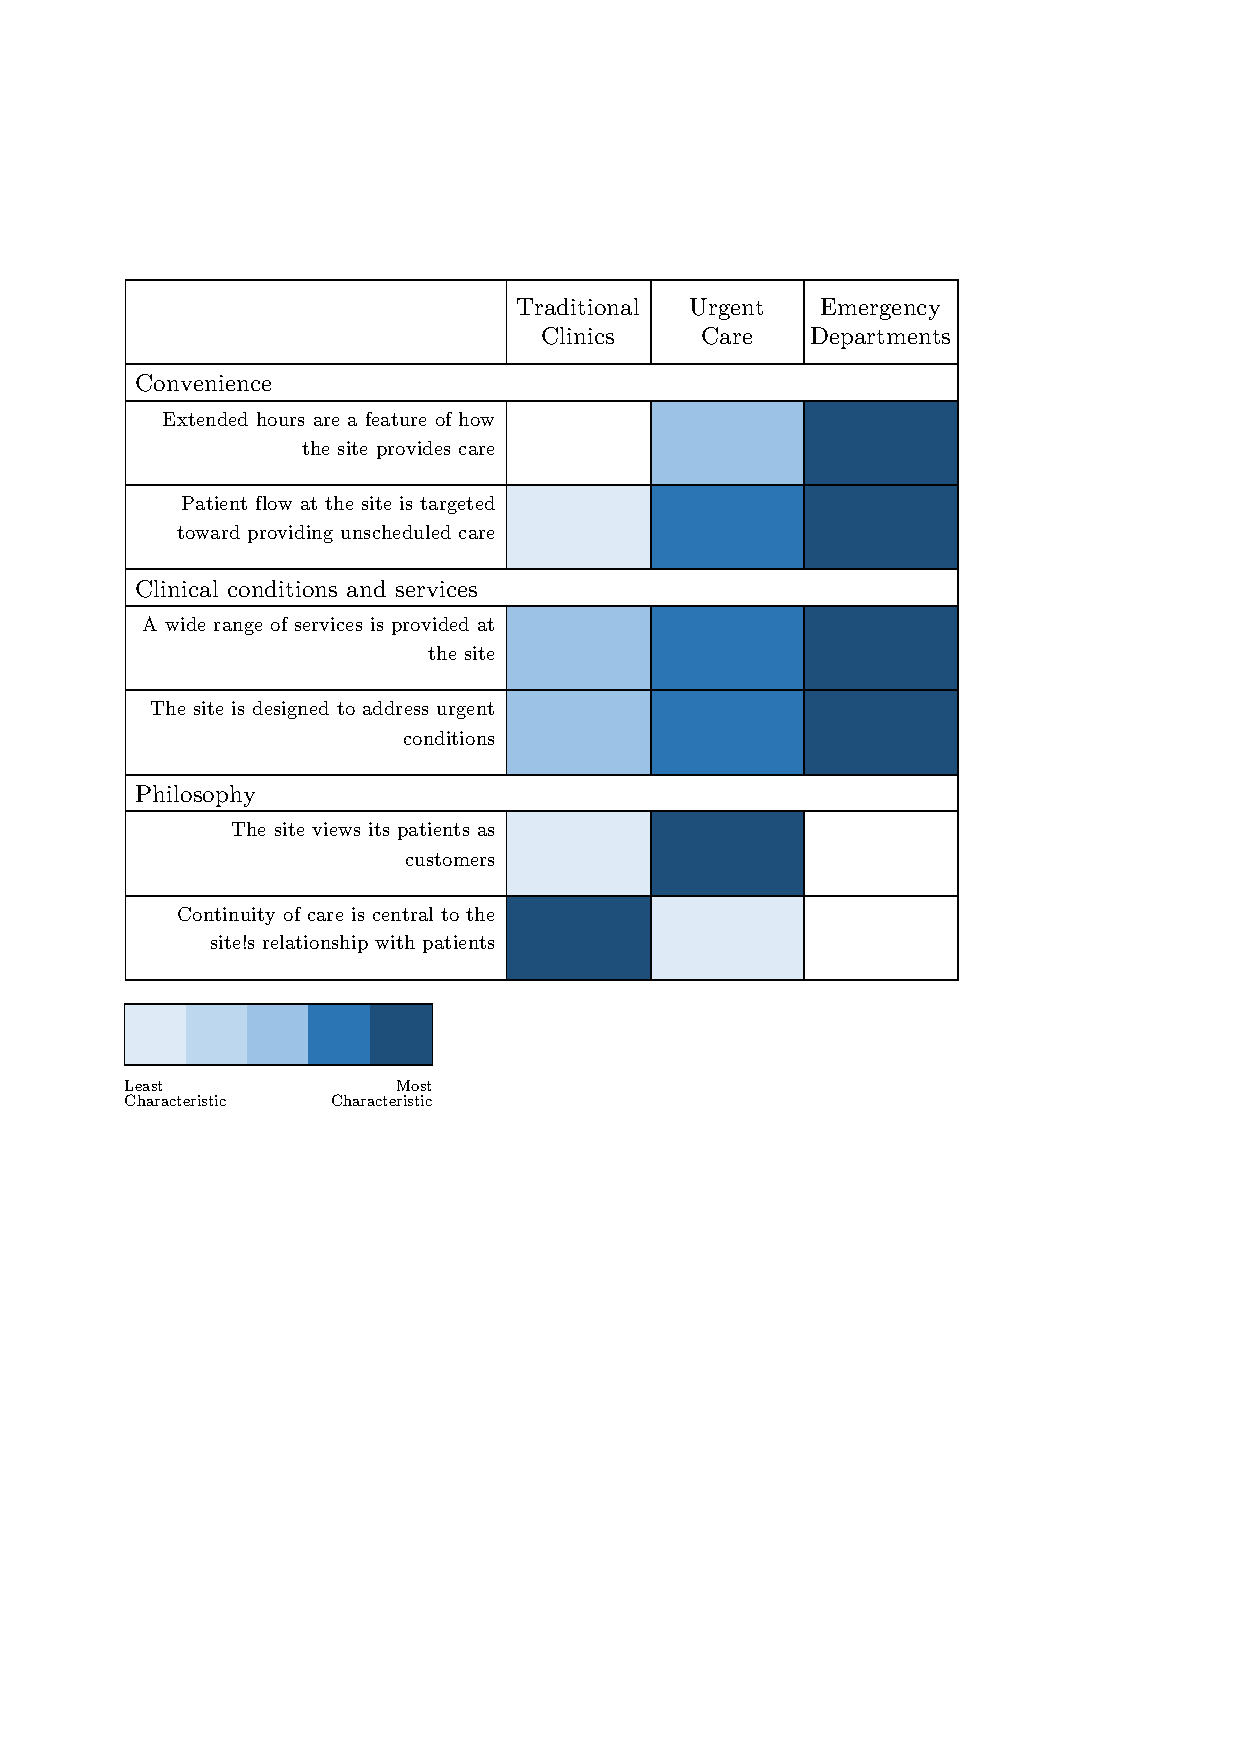
\includegraphics[scale = 0.75,angle = 0]{figures/table.pdf}
  \caption[Characteristics of Visit Sites]{\normalsize{Characteristics of Visit Sites}}
  \label{fig:tab1}
  \end{figure}
  
  As summarized above, this clearly orients urgent care facilities towards
  an acuteThough this is the acceptable definition of urgent care, it is
  important to not that much of this conceptualization of the industry has
  not caught up to the rapid changes taking place. The report took place
  in 2011, and even the past 3 years have seen
  
  \section{The Changing Fate of Primary
  Care}\label{the-changing-fate-of-primary-care}
  
  \begin{center}\includegraphics{Thesis_Skeleton_files/figure-latex/make_fig-1} \end{center}
  
  \begin{verbatim}
  NULL
  \end{verbatim}
  
  \section{Examining Trends: Fact or
  fiction}\label{examining-trends-fact-or-fiction}
  
  In the following analysis, I will attempt to situate the rise of such
  clinics within the existing sociological research on the American
  healthcare system, the changing face of primary care, and the patients
  that utilize it, examining hypotheses about how the patterns of use by
  patients at urgent care centers can help us understand and situate them
  in to the larger body of medical sociological research. To do this, I
  draw from theories on the changing relationship between the patient and
  practitioner to compare three hypotheses of urgent care usage.
  
  In Chapter one, I situate the analysis into the wider body of
  literature, emphasizing how structural changes in healthcare have
  generated profound consequences for primary care and modern patients. I
  begin to place urgent care centers into the context of the US healthcare
  system's varied actors and organizations, and explore the ways this
  method of care appears in the literature. In particular, the chapter
  highlights how these new organizations might informally facilitate the
  depersonalized relationship between practitioner and patient,
  eliminating the close ties many historical medical sociologists
  identified as vital to an optimal doctor patient relationship. Lastly, I
  identify the current gaps in the literature surrounding new forms of
  privatized medical care facilities which have been largely overlooked by
  sociologists and other scholars attempts to understand health care in
  America.
  
  Chapter two focuses strictly on urgent care centers themselves, and uses
  sociological theory to present three plausible explanations of urgent
  care usage. While the goal is not to generate a predictive model of
  urgent care, an analysis which tests the three hypotheses by examining
  sub-groupings of patients who visited urgent care goes far to allowing
  us to recognize identifiable medical use patterns. Chapter three offers
  a description of the National Ambulatory Medical Care Survey where I am
  drawing my analysis from, and includes a description of the methods I
  use to examine patient visits to urgent care. These include both a
  k-modal hierarchical clustering exploratory analysis used to identify
  groups of similar patients who used urgent care and a logistic analysis
  of those choosing to use urgent care as their primary care facility.
  Chapters four and five present these analyses, and discuss the findings
  in light of the research.
  
  In the conclusion, I explore the implications of the tensions between
  what is thought important to the doctor-patient relationship, and the
  reality of accessing healthcare in America today. I argue that primary
  care, while no longer the traditional town doctor, is still a key
  gateway for patients, and that urgent care centers may just be a new
  entry point into the traditional model. I conclude with implications and
  suggestions for further studies of urgent care and primary care access
  in America.
  
  \chapter*{Theoretical and Historical
  Foundations}\label{theoretical-and-historical-foundations}
  \addcontentsline{toc}{chapter}{Theoretical and Historical Foundations}
  
  \setcounter{chapter}{2} \setcounter{section}{0} \doublespacing
  
  In this chapter, the quantitative exploratory analysis of urgent care
  centers that follows later will be located in the long-term primary care
  trends of patients seeking care within the American healthcare system.
  To comprehend the how and the why of the proliferation of urgent care
  centers, one must have some understanding of the complicated and tangled
  history of the medical profession in the US, and how institutional
  changes and epistomological shifts have led to the current state of
  affairs. The existing sociological research on the patient and
  practitioner, and the evolution of this relationship, are vitally
  important to beginning to understand how and at what level urgent care
  centers may be operating, since changes in the last half century have
  had drastic effects on this relationship.
  
  \emph{I begin by tracing the development and subsequent decline of
  medical professional autonomy, paying particular attention to how
  structural changes dismantled the stronghold of political, economic and
  social power the profession claimed at its peak. I then review the
  current literature regarding the consequences of such structural changes
  on the doctor/patient relationship in the 21st century, taking up the
  traditional primary care physician's historical social importance.
  Combined, these changes lead us to the current ontologies of the
  American healthcare sphere where we will attempt to situate the role of
  urgent care centers and the patients who use them.}
  
  \emph{edited}
  
  I begin by examining patient choice through a sociological lens, paying
  particular attention to how the literature understands the factors which
  influence the ways that patients access primary care. From this, I turn
  towards an exploration of primary care itself, and its importance and
  role in the larger healthcare field, its influence on literature around
  the patient/physician relationship, and the importance of the
  traditional primary care physician's historical social role. An
  examination of the profession shows a clear peak and subsequent decline
  in the power of the primary care's professional dominance in recent
  years and their primacy in the foctors which influence patient
  decisions, and the last portion of the background examines how
  structural changes may have helped to both dismantle the stronghold of
  political, economic and social power of the primary care physician, and
  what effect this may have on modern patients seeking primary care at
  urgent care centers.
  
  \section*{Patient Choices}\label{patient-choices}
  \addcontentsline{toc}{section}{Patient Choices}
  
  \textbf{REALLY IMPORTANT SHIT}
  
  The last 30 years have seen a reconfiguration of the patient from
  passive recipient of care from their doctor to a critical consumer of
  health services (Barker 2008; Lupton et al. 1991; Timmermans and Oh
  2010). Theories of medical consumerism developed from economists
  studying the healthcare sector, and they begin with a similar hypothesis
  as the economic rational choice model, assuming that patients act as
  rational actors in the context of a medical encounter (Timmermans and Oh
  2010). In other words, individuals act in a calculated manner to engage
  in self-improvement or health, and they are generally skeptical about
  expert knowledge (Lupton 1997).
  
  \emph{Origins of the changing patient} According to the literature, this
  trend began to express itself in the form of solicitation of second
  opinions and a sense of interchangeability of medical practitioners
  during the 1980's, just as distrust of the industry reached its peak
  (Gray 1997). The idea that patients could shop around and compare
  services and prices was heavily popularized, and patients increasingly
  began to make autonomous decisions when selecting physicians (Hibbard
  and Weeks 1987; Lupton et al. 1991).
  
  Urgent care centers fit neatly into such a conceptualization of health
  services, and thus offer a key area of analysis in better understanding
  the developing roles of the consumer-patient within the larger
  healthcare industry. An important aspect of the research on the
  developing patient-consumers emphasizes the expansion of bargaining
  power on the part of the patient that came with the shift (Reeder 1972).
  A patient may now shop around the marketplace of health care, and that
  many are now choosing urgent care centers is undeniable given the
  industry's rapid expansion.
  
  The shift towards urgent care centers undoubtedly plays some part in the
  transformations of the patient-practitioner relationship and the
  patient's role in the medical care system discussed above, but so far
  these consequences remain largely unknown. Fortunately, sociologists
  have had a long-standing concern with such professional-client
  interactions, particularly within medicine (Freidson 1961; Mechanic
  1966), and in order to better understand what effects the shifting norms
  around primary care physicians may have on patients, one can look to a
  large body of research on how institutional and organizational
  environments directly affect a patient's experience in health care.
  
  In 1963, Samuel Bloom published what would become one of the most cited
  sociological texts on the relationship between physicians and patients
  (Bloom 1965). Even the title implies a power imbalance: the patient
  belongs to the doctor, whom distrbibutes his expert knowledge which is
  taken by the patient as truth on the basis of the profession's
  techno-cratic authority.
  
  Most of the literature locates the stability of this doctor-patient
  relationship in the fact that the physician acts as the patient's agent,
  yet one can immediately recognize that urgent care centers may not be
  equipped to facilitate this relationship in the same way that the
  traditional primary care practice is seen to (Lupton 1997). The premise
  of urgency in such practices, the quickness with which patients are
  seen, and the targeted focus on acute problems all serve to create
  considerable doubt towards the ability of physicians within such an
  organizational context to fulfill the sociological role thought so
  important in previous literature.
  
  Additionally, those who study health services have recognized that a
  patient's medical history is a primary source of information regarding
  treatment, and primary care practitioners have been known to draw upon
  this as a valuable resource (Draper and Smits 1975; Miller et al. 2010).
  Urgent care centers however have no emphasis on maintaining
  patient-doctor ties and there is no reliable system to ensure a patient
  sees the same doctor even if they have been there before.
  
  \subsection{Why maight patients not choose a traditioanl primary care
  practitioner?}\label{why-maight-patients-not-choose-a-traditioanl-primary-care-practitioner}
  
  \emph{Look into what makes a patient choose to opt out of a traditional
  care model?}
  
  Turning away from the fate of doctoring, it is important to acknowledge
  that the fate of primary care physicians has been reported to be hanging
  in the balance for quite some time. In 2005, the American College of
  Physicians released a report with the ominous title ``The Impending
  Collapse of Primary Care Medicine and Its Implications for the State of
  the Nation's Health Care'' (2006). Yet while this may seem troublesome,
  a large body of recent sociological literature belongs to a growing
  number of scholars who are challenging the importance, and even
  relevance, of the traditional primary care physician in modern medicine.
  Those who have been observing developments in the patient-physician
  relationship over the past 30 years argue that the last quarter of the
  20th century saw a dramatic reconfiguration of society, especially in
  regards to health services, which has had profound effects on an
  individual's relationship to the healthcare system. So while some were
  witnessing what was, for Starr (1982), ``the social transformation of
  medicine,'' and for many, ``the end of the golden age of doctoring''
  (McKinlay and Marceau 2002).
  
  \section*{\texorpdfstring{The Rise and Fall of the \emph{Golden Age of
  Doctoring}}{The Rise and Fall of the Golden Age of Doctoring}}\label{the-rise-and-fall-of-the-golden-age-of-doctoring}
  \addcontentsline{toc}{section}{The Rise and Fall of the \emph{Golden Age
  of Doctoring}}
  
  Since sociologists' initial interest in studying medicine and
  healthcare, the discipline was deeply intertwined with studies of the
  sociology of professionals and professionalism. In the U.S., Doctors
  were seen as the paragon of the \emph{professional}: respected,
  organized, in control, and above all else, firmly established in their
  positions. Such traits led many to study what effects this had on
  medical care and how such professional dominance of medical
  practitioners shaped what services were provided. Many found that such
  dominance allowed the profession to block off areas of study entirely,
  or to ignore diseases they did not want to pursue. Such ``modern
  doctors'' worked within a ``sovereign profession'' (Starr 1982),
  serenely dispensing both medical care and authoritative judgment.
  Freidson comments that before the 1970's, U.S. medicine ``was at a
  historically unprecedented peak of prestige, prosperity and political
  and cultural influence---perhaps as autonomous as it is possible for a
  profession to be''(1988, p.384).
  
  At the center of this prestige was the Physician. In the traditional
  Parsonian model, the Physician treated patients according to generalized
  technical standards of treatment (universalism), enacted a specific
  technical focus on medical care (specificity), treated patients without
  emotional investment (affective neutrality), and put the patient's
  welfare above their personal interests (the `collective' orientation)
  (Parsons). Of course, even Parsons himself noted this was meant to
  function as a highly abstract view of the physician (1951, p.440), yet
  even in summary it bestows upon the doctor the scientific and moral high
  ground that was at one point firmly ingrained in the American psyche.
  
  Similar views of the doctor occur profusely throughout early to mid
  twentieth century literature on the profession, and is even visible
  today, though often as either a past to be reminisced on, or a goal to
  be returned to. A person's doctor, traditionally, was an extremely
  integrated, close, and important connection in a person's life. This was
  a relationship built, for some on trust, agency, and mutual
  understanding, while for others on power imbalance, technocratic
  authority and affective neutrality. When one thinks of the healthcare
  industry today, it is hard to call to mind the professional cohesion
  previously discussed. While doctors remain one of the more highly
  respected career choices in America, their prestige has certainly
  dropped since the 20th century (Heritage and Maynard 2006). The term
  doctor is now applicable to a wide variety of sub-professions and
  specialties and the medical profession has become extremely diversified.
  While this may not have necessitated a drastic change in the societal
  role of the doctor, social scientists interested in this changing
  relationship have identified many possible sources of erosion.
  
  \subsubsection*{The 21st century state has switched
  sides}\label{the-21st-century-state-has-switched-sides}
  \addcontentsline{toc}{subsubsection}{The 21st century state has switched
  sides}
  
  The government was an active and powerful ally in the rise of the
  medical profession during the 20th century (Alford, 1975). Political
  policies and government agencies served as buffers against what was
  `legitimate' medicine and what was not, reaching the point where
  physicians achieved an almost monopolistic power over medical care. More
  than any other profession, the state served as legitimator and ally to
  medical professionals: state licensing for example, made it impossible
  for any other health care provider to legitimately practice medicine
  (Freidson, 1970a).
  
  According to the literature, all of this began to unravel around the
  turn of the century, and in recent years the state has been
  transitioning towards an anti-leviathan New Right viewpoint, no longer
  supportive of health care (McKinlay \& Marceau, 2002). This new approach
  avoids government intervention in economic and social life, consequently
  shifting the support of the state from the established medical
  organizations towards private interests. This shift in the primary
  allegiance of the state is reflected in many areas of social policy and
  has been clearly illustrated in recent attempts at health care reform,
  such as the Afforable Care Act.
  
  Along with the government alliance shifts, big changes to Medicare and
  Medicaid legislation and the growth of third-party payers and for-profit
  medical service corporations created conditions which further removed
  the doctor from their traditional roles, eroding the political and
  cultural influence of the profession and threatening the cultural
  authority and technical autonomy of medicine (Starr 1982, Freidson
  1988).
  
  \subsubsection*{Epidemiological
  transitions}\label{epidemiological-transitions}
  \addcontentsline{toc}{subsubsection}{Epidemiological transitions}
  
  Interestingly, one of the other most cited causes of the decline of
  primary care physicians, both in numbers and in prestige, is what is
  known as the epidemiological transition of developed countries (McKinley
  2008). Medicine's rise around the middle of the 20th century coincided
  with the tail end of the infectious disease era. While there is academic
  disagreement over whether this decline was the result of medical
  organizations or an overall economic development, what is clear is that
  standards of living started to rise and Americans began to get sick
  \emph{differently}. Rather than infectious diseases, which could strike
  anyone at any time, many argue that America has entered into a new
  epidemiological phase of chronic illness. According to one estimate,
  within 5 years (2020), an estimated 75 million Americans will have at
  least one chronic condition (Wu \& Green, 2000).
  
  While some could imagine that such chronic illnesses could secure the
  position of the primary care physician, McKinley argues that the new,
  chronically ill patient base is different in a fundamental way: ``A well
  informed patient population can now obtain a proxy diagnosis on-line, or
  through health risk appraisals'' (2008, p.~1483). Many patients know, or
  at least strongly suspect their ailment before ever considering a doctor
  and, according to McKinley, may even skip the initial diagnosis all
  together and immediately seek out a specialist.
  
  \subsubsection*{Expansion of the playing
  field}\label{expansion-of-the-playing-field}
  \addcontentsline{toc}{subsubsection}{Expansion of the playing field}
  
  Similarly to the retraction of government involvement, the last half of
  the 20th century saw a major expansion of health care actors. Physicians
  had the medical playing field almost entirely to themselves for most of
  the beginning of the 20th century, but this was no longer true as early
  as the 1970s. Non physician clinicians, unheard of 40 years ago, have
  increased dramatically in number, and what was once the sole field of
  the physician is now occupied by a range of actors (Starr, 1982; Cooper,
  Laud, \& Dietrich, 1998).
  
  This is where urgent centers enter into the game most clearly: Late 20th
  century changes in the organization and financing of U.S. health care
  opened the door for the emergence of profit driven corporate care, and
  created a labor market for non-physician clinicians. For clinics which
  can staff a nurse practitioner for a fraction of the cost of a doctor,
  the choice is clear. Lower costs and customer satisfaction (two of the
  major tenets of the urgent care model) are widely accepted as 21st
  century health care priorities, and the result has been a dramatic surge
  in the competitive medical marketplace for health care.
  
  It should be noted that such changes may not have necessitated a loss of
  professional dominance. In fact, with the expansive growth on spending
  in the healthcare sector that the last 30 years have seen, it is
  plausible to imagine that doctors could have further cemented their
  professional medical authority. But most scholars have observed that the
  opposite has happened, and instead many view the past 30 years as the
  end of the authoritative medical professional.
  
  \section*{From patient to client}\label{from-patient-to-client}
  \addcontentsline{toc}{section}{From patient to client}
  
  These shifts in the professional dominance of the medical professional
  occurred parallel to changing norms surrounding the roles of both
  patients and practitioners, all of which directly affect a patient's
  acquisition and utilization of primary care. In 2006, the Millis report,
  commissioned by the American Medical Association, was asked to review
  the current status of physicians in the US. In the first section, they
  recalled the coveted physician of memory in America:
  
  \singlespace
  
  \begin{quote}
  ``The general practitioner of revered memory knew his patients\ldots{}
  and provided continuing care through the course of minor ailments and
  majors emergencies. His deficiencies\ldots{} were partly offset by
  intimate knowledge of his patients, the support he gave them, and the
  trust and confidence his services engendered.''
  \end{quote}
  
  \doublespacing
  
  Intimate knowledge like that of a family practitioner who has known his
  patients for years is, according to both sociological and psychological
  research, the basis of a functional and stable doctor-patient
  relationship. A major sociological conceptualization of such
  relationships begins by speculating that the bureaucratization of modern
  social institutions has had drastic consequences on an individual's
  relationship to others and healthcare: as opportunities for close
  personal contacts diminish, problems which were originally handled in
  familial, social, and religious contexts are said to be transferred to
  `formal sustaining practitioners' (Mechanic 1966). In modern societies,
  the prescribed structure of the `doctor' and the `patient' then provides
  a legitimization for the expression of intimacy and the request for help
  (1996). In other words, along with physical complaints and ailments,
  patients have coexisting and equally important socio-emotional needs,
  and sociologists of medicine have viewed addressing these needs as an
  essential task of the primary care physician.
  
  But transformation is visible here as well: the ``doctor'' has become a
  ``provider'', the patient a ``cliet''. Juhar (2006) uses this ``demise
  of the Physical Exam'' as an illustration of these changing roles. He
  believes that patient testing technologies used in modern clinics are
  the newest in a long line of technologies and codified procedures which
  allow for \emph{diagnosis at a distance}. Markel (2006, p551) agrees
  with Jauhar, and presents the stethoscope as the best symbol of medical
  practice, ``\ldots{} it embodies the essence of doctoring: using science
  and technology in concert with the human skill of listening to determine
  what ails the patient.''
  
  But he points out that, prior to the stethoscope, physicians would place
  an ear directly against a patient's chest, a practice which inspired the
  inventor of the stethoscope only in that he found the act `disgusting'
  and fashioned a listening technology which he could use to listen from a
  distance. Markel goes on to suggest that it was perhaps the stethoscope
  that began the process of physically separating physicians from their
  patients, and that with the rise of noninvasive imaging and testing and
  remote technologies, that distance will only continue to grow (2006).
  
  \subsection*{Consequences for health
  care?}\label{consequences-for-health-care}
  \addcontentsline{toc}{subsection}{Consequences for health care?}
  
  In light of such research, those who study at the intersection of health
  and social behaviors have begun to re-examine the importance of a
  close-tie relationship between doctor and patient in an attempt to
  respond to the consumer-patient model, developing a growing body of
  research which seeks to define the most effective components of
  patient-physician interactions and to reaffirm the place of the primary
  care physician in modern medicine. Common to most of these studies are
  the elements of `trust, compassion, communication, and clinical
  competence' (Heritage and Maynard 2006; Phillips and Bazemore 2010,
  others at bottom). As an example, a 2002 study on clinical outcomes for
  low income women over the age of forty found that women who rated
  highest their doctor's ability to take care of all of their health care
  needs had 11 times the odds of `trusting their physician' and 6 times
  the odds of finding their physicians `compassionate and communicative',
  compared to those with the lowest level of comprehensiveness (O'Malley
  and Forrest 2002).
  
  With the knowledge that close ties between physicians and patients have
  a direct impact on the perceived quality of care, the importance of
  examining the rise of urgent care centers become obvious. If patients
  are acting as rational consumers, which of them are choosing to receive
  their care outside of a primary care office, and what consequences does
  this have for their medical outcomes? The lack of research into the
  characteristics of urgent care patients make it difficult to answer such
  questions. Indeed, as of now, there has been no academic attempt to
  place the rapidly growing industry within the sociology of medicine, nor
  does there even exist an official definition of what constitutes an
  urgent care center.
  
  In the next section, three opposing hypotheses are developed regard how
  urgent care centers play a role in this new patient decision-making
  process.
  
  \chapter*{Model Building: theories of urgent care
  use}\label{model-building-theories-of-urgent-care-use}
  \addcontentsline{toc}{chapter}{Model Building: theories of urgent care
  use}
  
  \setcounter{chapter}{3} \setcounter{section}{0} \doublespacing
  
  Urgent care centers are an obviously understudied phenomenon in modern
  medicine, and the following section applies the sociological background
  discussed in the last chapter to better understand their role in the
  healthcare system and why patients might choose to pursue primary care
  at such facilities. The conceptualization of urgent care as a new source
  of primary care for patients is contrasted against two other theories of
  urgent care center usage. The first applies theory to the widely
  matriculated explanation of urgent care by the media and health
  economists: that urgent care is a response to unavailability in primary
  care, developing out of consumer demand for quick and cost-efficient
  care. The second draws from the sociological research that focused on
  emergency departments (an oft cited cousin of urgent care centers), and
  explores the possibility that the industry has developed as a response
  to overcrowding and overuse of emergency departments in the past 20
  years.
  
  \section*{H1: An extension of the Welfare
  State}\label{h1-an-extension-of-the-welfare-state}
  \addcontentsline{toc}{section}{H1: An extension of the Welfare State}
  
  The prevailing theoretical understanding of urgent care centers
  interprets the industry's growth as a development that came out of
  emergency department overcrowding that began during the financial
  tightening of the 1980's. Thus, each clinic is often conceptualized as a
  smaller instance of a traditional hospital's triage center, supplying
  many services which one could receive at an emergency department (Anon
  n.d.; Mehrotra et al. 2008; Rubin 2012). One study which compared
  emergency department services with urgent care centers found that, for
  all but the most extreme care and emergent care needs, urgent care
  centers could handle almost all of emergency department traffic and that
  their services were remarkably analogous (Anon n.d.). Similarly, the
  unique features of emergency departments which set them apart from more
  traditional avenues of care such as the promise to be seen regardless of
  insurance coverage and the flexible hours are mirrored in most urgent
  care centers (Weinick and Betancourt n.d.).
  
  Given these similarities, urgent care could in many ways be considered a
  response by the healthcare industry to emergency department overuse,
  which continue to struggle underneath a lack of resources. Suitably, the
  body of sociological research on emergency departments can be used to
  better comprehend how urgent care centers are impacting the allocation
  of healthcare. Many medical sociologists have analyzed the
  public/private divide in the healthcare industry, emphasizing the
  unequal quality of care received depending upon which type of health
  service you utilize (Dutton 1978; Luftey and Freese 2005). In response
  to these inequalities in the private sector, the emergency room has long
  been understood as a response to a stratified system, and it is largely
  considered a social welfare institution (Gordon 1999). ``The hospital
  emergency department is perhaps the only local institution where
  professional help is mandated by law, with guaranteed availability for
  all persons, all the time, regardless of the problem'' (Ullman, Block,
  and Stratmann n.d.), and was for a long time widely considered one of
  the few access points into the healthcare system for very low income
  individuals.
  
  Accordingly, because urgent care centers offer a similar alternative to
  primary care for those who cannot procure a conventional family
  practitioner, they can be considered an extension of a much needed
  welfare institution necessary to circumvent an extremely stratified
  healthcare industry. This becomes more credible when trends in urgent
  care centers are examined in conjunction with emergency departments. By
  all indications, the demand for emergency departments far outweighs
  their capacity, and this is only expected to grow in the future (Weinick
  2010). Around the time that urgent care centers began to emerge in the
  U.S., emergency departments were seeing record breaking levels of
  non-acute visits, resulting in severe overcrowding and shortages
  (Shortcliffe). These numbers have only risen in the past 20 years,
  especially in urban areas with large populations of low-income residents
  (Anon n.d.). Not only does this rise in demand correspond to the growth
  of the urgent care industry, one economic analysis which took cities
  with comparably high levels of non-emergent ED usage and examined the
  effect of a growing number of urgent care centers found that cities
  which have seen a large growth in these facilities have statistically
  lower overcrowding in emergency departments (O'Malley 2013).
  
  Thus, urgent care centers usage would be expected to closely resemble
  that of the emergency department, especially regarding non-emergent
  care. This leads to the first hypothesis which will be tested by current
  data on urgent care center usage. Emergency department usage has been
  studied by many medical professions and sociologists, with a particular
  focus on the ways in which it serves as a welfare institution, and a few
  central patterns will be used here in the comparison with urgent care
  centers. Primarily, the low average income of patients and high levels
  of uninsured visits to emergency department patients have been a steady
  trend in the last 30 years (Ullman et al. n.d.). Patterns of use for
  emergency departments also show low levels of `returns' (individuals who
  come back with the same problem) and higher traffic during hours when
  normal primary care physician offices are closed, such as late at night
  and on the weekend (Anon n.d.; O'Malley 2013; Ullman et al. n.d.).
  Accordingly, if like emergency departments, urgent care centers act as a
  a welfare institution for those who cannot procure a traditional primary
  care physician, we would expect to see similar trends as have been
  observed in hospital emergency departments. These are summarized in
  Hypothesis 1 below.
  
  \begin{quote}
  Hypothesis 1: \emph{Urgent care centers will experience high levels of
  visits from uninsured and low SES patients, have low rates of second
  visits, and higher rates of visits during non-traditional hours
  (weekends).}
  \end{quote}
  
  \section*{H2: Response to Consumer
  Disatisfaction}\label{h2-response-to-consumer-disatisfaction}
  \addcontentsline{toc}{section}{H2: Response to Consumer Disatisfaction}
  
  What work has been done to understand the expansion of urgent care
  centers has largely accounted for them by citing the growing
  dissatisfaction and impatience of privately insured Americans who's
  primary care physicians are very difficult to reach. Such a view
  conceptualizes urgent care centers as a market response to the demand
  created by middle to upper class Americans with minor ailments and low
  level of patience. It holds that, due to the well-known emergency
  department issue of over-crowding (largely a consequence of hypothesis
  1), urgent care centers were a demand made by the individuals attempting
  to avoid the emergency room. This also happens to be the most well cited
  reason for urgent care's popularity.
  
  Basically, hypothesis 2 conceptualizes the urgent care center as an
  occurrence of boundary work by upper middle class and wealthy Americans
  who have been pushed out of emergency departments by low SES patients.
  Sociologists have long been interested in the ways that class can be
  defined and reconstituted through boundary work (Pachucki, Pendergrass,
  and Lamont 2007). Research on symbolic boundaries---the conceptual
  distinctions made by social actors in categorizing people, practices,
  tastes, attitudes and manners---and their interactions with more durable
  and institutionalized social differences such as class and race has
  shown that individuals often use methods of exclusion through
  organizational settings in order to solidify social boundaries Zietsma
  and Lawrence 2010.
  
  Thus, if it is true that urgent care centers are largely operationally
  analogous to emergency departments as is often observed, it could be
  that such organizations serve as an alternative for wealthy individuals
  who seek to socially distance themselves from a space largely inhabited
  by low SES patients. Such a hypothesis would explain why the industry's
  rapid growth coincides with a remarkable strain on emergency
  departments' capacities due to an influx of low SES patients. This
  explanation also accounts for the fact that urgent care centers are
  often more expensive due to their pay-per-service model than emergency
  departments (Anon n.d., Anon n.d.; Ullman et al. n.d., n.d.). Lastly,
  this theory offers an explanation as to why urgent care centers have
  developed along side of, and with many of the same services as,
  emergency departments Weinick et al. 2009.
  
  If this hypothesis were the case, one would expect to observe usage
  trends much like Hypothesis 1, but with key differences. Primarily,
  regardless of insurance coverage, we should expect to see little to no
  low-SES users in such clinics. We would also expect to see patterns of
  use by the wealthy to mimic their would-be use of emergency departments,
  such as high volumes of visits during times when their primary care
  physicians are closed, emergency and injury related visits and almost no
  return visits.
  
  \begin{quote}
  Hypothesis 2: \emph{Urgent care centers will experience high levels of
  visits from high SES patients, have low rates of second visits and will
  have large proportions of visits which qualify as acute and emergent
  care during non-primary care hours.}
  \end{quote}
  
  \section*{H3: New Model of Primary
  Care}\label{h3-new-model-of-primary-care}
  \addcontentsline{toc}{section}{H3: New Model of Primary Care}
  
  Yet another understanding of urgent care centers arises when one
  considers the larger institutional context within which the overuse of
  emergency departments and the boom in the urgent care industry occurred.
  According to medical and organizational sociologists, the institutional
  narrative of the American healthcare industry since the 1980's is one of
  privatization and the transfer of power from professionals and the
  government towards the private sector and market control (Waitzkin
  2000). Urgent Care centers thus fall into a rapidly expanding category
  of new, privately funded modes of healthcare services---other examples
  being retail clinics, private hospitals and home care
  organizations---which are provided and predominantly paid for by private
  actors (Anon n.d.).
  
  This framework has yet to be fully examined by scholars, but a few
  studies which have attempted to examine the place of urgent care centers
  in new healthcare markets have pointed towards such change as being
  highly indicative of larger changes to healthcare, highlighting the
  privatization phenomenon as a possible explanation in the rise in
  numbers of such clinics over the last two decades or so (Rubin 2012;
  Weinick, Bristol, and DesRoches 2009; Yee et al. 2013). Shortages in
  public hospital staffing and facilities and the rising cost of care in
  the U.S. are seen as having created both demand and an opening for a new
  market within healthcare, which has been filled by new forms of medical
  service (Weinick and Betancourt n.d.). And while the trend towards
  privatization has been seen at times as both a symptom of the loss of
  professional dominance by medical practitioners and the cause of it, the
  similarities in organizational structure to primary care practices cast
  doubt on the hypothesis that these new forms of care are simply
  emergency department overflow. As one analysis observed: ``while urgent
  care reflects some similarities to emergency departments, we find that
  in other areas -- most notably reimbursements, primary payer
  distribution, and physicians' salaries -- urgent care centers seem far
  more similar to office-based family medicine practices'' (Weinick and
  Bristol 2008).
  
  Such observations lead one to a different conclusion about urgent care
  than those who liken the clinics to smaller triage centers created to
  handle emergency department overflow. Instead, urgent care centers can
  be conceptualized as a move by the healthcare industry towards deeper
  privatization, and possibly a response to medical professional authority
  in jeopardy. When medical sociologists first began pointing to ``the end
  of the golden era of doctoring,'' Stefan Timmermans responded by
  pointing to the long history of adaptability by the medical profession,
  which has managed to transform itself before in the wake of
  institutional change many times before (Timmermans, Whooley).
  
  Consequently, if the privatization of healthcare proves to be the
  primary explanation of why urgent care centers are beginning to dominate
  the acute-care market, one would expect to see trends in use mirror
  those of traditional primary care physicians rather than emergency
  departments. Historically, primary care often acted as a first contact
  point for insured patients for any acute, non-emergent health concerns
  of these individuals (Jost 2003). While many primary care offices will
  accept at least a small number of Medicaid and Medicare payments, they
  often have a large patient base of privately insured, financially
  well-off individuals (Cunningham et al. 1999). Such offices are often
  only open during a standard work week's hours, a facet often noted as
  functioning to limit access for those who cannot take off work to go to
  the doctor. Lastly, primary care is often set apart from other forms of
  care due to the relationship and medical history that develops between
  the doctor and patient over years of care exchange (Miller et al. 2010).
  Primary care physicians thus emphasize holistic view of health care, and
  for those patients that do have a primary doctor, they are encouraged to
  return to the same clinic. If urgent care facilities are to be
  understood as a new face on a conventional sector of the health services
  industry, we should expect to see this last factor of primary care
  present in those going to urgent care centers. These usage trends are
  summarized in Hypothesis 2 below:
  
  \begin{quote}
  Hypothesis 3: \emph{Urgent care centers will experience high levels of
  visits from insured patients across SES statuses, have high rates of
  second visits, and will not have significantly higher rates of visits on
  weekends.}
  \end{quote}
  
  If such trends were observed, the urgent care center could then be
  understood as analogous to an emergency department for the wealthy.
  \autoref{tab:sumz} summaries the three hypotheses:
  
  \begin{longtable}[c]{@{}rl@{}}
  \caption{Summary of three hypotheses of urgent care centers'
  use.}\tabularnewline
  \toprule
  \begin{minipage}[b]{0.32\columnwidth}\raggedleft\strut
  Hypothesis
  \strut\end{minipage} &
  \begin{minipage}[b]{0.62\columnwidth}\raggedright\strut
  Expected
  \strut\end{minipage}\tabularnewline
  \midrule
  \endfirsthead
  \toprule
  \begin{minipage}[b]{0.32\columnwidth}\raggedleft\strut
  Hypothesis
  \strut\end{minipage} &
  \begin{minipage}[b]{0.62\columnwidth}\raggedright\strut
  Expected
  \strut\end{minipage}\tabularnewline
  \midrule
  \endhead
  \begin{minipage}[t]{0.32\columnwidth}\raggedleft\strut
  1: Welfare Apparatus
  \strut\end{minipage} &
  \begin{minipage}[t]{0.62\columnwidth}\raggedright\strut
  Low SES, Self-Pay/Uninsured, Return visitors
  \strut\end{minipage}\tabularnewline
  \begin{minipage}[t]{0.32\columnwidth}\raggedleft\strut
  2: Consumer Dissatisfaction
  \strut\end{minipage} &
  \begin{minipage}[t]{0.62\columnwidth}\raggedright\strut
  Med-High SES, Private Insurance, Weekends
  \strut\end{minipage}\tabularnewline
  \begin{minipage}[t]{0.32\columnwidth}\raggedleft\strut
  3: Primary Care
  \strut\end{minipage} &
  \begin{minipage}[t]{0.62\columnwidth}\raggedright\strut
  Med-High SES, Private/Gov Insurance, Business days
  \strut\end{minipage}\tabularnewline
  \bottomrule
  \end{longtable}
  
  An examination and comparison of these three models is to follow, and
  the results strengthen the trends discussed in the literature reviewed
  in the last chapter. While the direct effects of so many transitions in
  healthcare may not be immediately effective, this thesis attempts to at
  least show that the effects are experienced differently based on
  individual's life experience.
  
  \chapter*{Methods}\label{methods}
  \addcontentsline{toc}{chapter}{Methods}
  
  \setcounter{chapter}{4} \setcounter{section}{0} \doublespacing
  
  The primary goals of this analysis are to 1) offer a better
  understanding of the characteristics and use patterns of patients at
  urgent care centers and 2) to examine empirically the differences
  between these individuals and those who continue to use traditional
  means of healthcare. Given these dual interests, the analysis was
  performed in three stages. First, an exploratory cluster analysis was
  performed on an abundance of patient characteristics for those who were
  coded as having gone to urgent care centers. Second, the results of the
  cluster analysis were used to inform a logistic regression analysis
  which examines the significant indicators which have an affect on
  whether a patient will make the initial decision to go to urgent care
  over traditional primary care. Third, a secondary regression analysis
  was performed to determine differences between patients using urgent
  care as primary care and those who do not.
  
  \section*{Data}\label{data}
  \addcontentsline{toc}{section}{Data}
  
  An empirical exploration of the hypotheses proposed in chapter two
  requires data that provides an abundance of variables which may or may
  not be statistically important but which we cannot initially rule out,
  as well as a large sample size since the phenomenon is still
  comparatively rare when thinking about how patients access primary care
  in the US. Given these initial requirements, I chose the National
  Ambulatory Medical Care Survey (NAMCS), which is a national survey
  designed and distributed by the American Center for Disease Control
  (CDC) to provide researchers in the medical and social science fields
  ``accurate and reliable information about the provision and use of
  ambulatory medical care services in the United States'' (Anon n.d.).
  
  For those unfamiliar with healthcare lingo, ambulatory care is defined
  by the survey as health services or acute care services provided to
  patients on an outpatient basis (without an overnight stay). Once a year
  NAMCS surveys randomly selected visits to non-federal employed
  office-based physicians, which are collected from a representative
  sample of the United States' medical care facilities. These surveys
  record over 500 variables on information about how the patients utilize
  physician services, the conditions most often treated, and the
  diagnostic and therapeutic services rendered, including medications
  prescribed. Because it is both representative of the larger trends in
  the United States and includes specific information regarding urgent
  care centers which can be used to explore that health care trend in
  particular, the data set serves the purposes of the current study quite
  well.
  
  Some limitations to the data should be noted. There may be related
  errors given that as the popularity of urgent care centers have risen,
  so too have the number that participated in the NAMCS. In 2008, there
  were 842 visits surveyed compared to 1168 surveyed in 2010. There may
  also be a compounding factor of selection: many urgent care centers are
  classified as retail clinics by the CDC, and are thus not included in
  the NAMCS random selection pool. Even with these limitations, the CDC
  specifically offers the NAMCS as a tool for social scientists, and this
  analysis depends on their collection methods being statistically
  expandable.
  
  \section*{Variable Selection and Summary
  Statistics}\label{variable-selection-and-summary-statistics}
  \addcontentsline{toc}{section}{Variable Selection and Summary
  Statistics}
  
  The NAMCS is a large data set: compiling observations for the years
  2008-2012 generated a data set of over 100,000 observations with 547
  variables. In order to explore such a large amount of data, I began the
  analysis by utilizing unsupervised statistical learning methods in order
  to develop descriptive categories of urgent care center patients. The
  advantages of performing an initial analysis of this nature are its
  ability to efficiently examine a large amount of variables and highlight
  those that should be included in later analyses. This choice was
  motivated by the current lack of statistical analysis and social theory
  surrounding urgent care centers, which makes it difficult to develop a
  model from scratch. The results of the clustering act as a guide for the
  regression techniques by identifying variables with some relationship to
  urgent care.
  
  For the clustering, I examined the group of visits which were coded as
  having been at ``Urgent Care Centers/Freestanding Clinics'' by the
  NAMCS. While the combined years produced a data set of 123,120
  observations, only 3,863 of those occurred at urgent care centers (about
  3 percent). Of these visits, I limited the analysis to observations
  without missing information, bringing the sample to 3,695 visits to
  urgent care centers. \emph{insert table 3.1}
  
  \section*{\texorpdfstring{\emph{k}-Modes Cluster
  Analysis}{k-Modes Cluster Analysis}}\label{k-modes-cluster-analysis}
  \addcontentsline{toc}{section}{\emph{k}-Modes Cluster Analysis}
  
  This method allows for grouping patients that have similar
  characteristics across a set of variables by dividing a set of cases
  into ever more numerous and specific subsets, thus leading to
  homogeneous empirical types (Rapkin and Luke, 1993). One of the most
  powerful exploratory aspects of cluster analysis is that you do not need
  to have a response variable in order to better understand your data. For
  this project, this is extremely useful since we initially only know who
  is going to urgent care and who is not, but would like to understand
  them as a group better before drawing comparisons between patients who
  visited a traditional primary care clinic. Another advantage for cluster
  analysis is that since such inductive methodologies are based only on
  quantitative similarities among cases, only two factors may be
  responsible for trends in the data: the actual structure of the observed
  phenomenon and the methodological decisions I made concerning choosing
  the cases and variables (including the statistical method used to
  identify subsets). A further explanation of the \emph{k}-modes
  clustering performed on the data is available in Appendix 1.
  
  Because I am interested in two somewhat distinct aspects of the patients
  of Urgent Care -- both their demographics and their patterns of use --
  The clustering was performed in two batches of parameters. Variables for
  \emph{Age, Sex, Race, Urban Type, \% Neighborhood Poverty, \%
  Neighborhood college degree attainment, and Payment Type}, what I will
  refer to as the \emph{demographic variables} from this point forward,
  were first analyzed for subgroups. Secondly, some of the same variables
  were again analyzed with the behavior parameters of \emph{Injury related
  visit (y/n), Primary Caregiver, Seen Before?, Past Visits, Major Reason,
  and the day of the week}, what I will refer to as the \emph{behavior
  parameters}. The summary statistics for these variables can be found in
  Table 1 of Appendix 2.
  
  \subsubsection*{Patient and Visit
  Characteristics}\label{patient-and-visit-characteristics}
  \addcontentsline{toc}{subsubsection}{Patient and Visit Characteristics}
  
  Many of the variables chosen to include in the exploratory cluster
  analysis were selected with both an awareness of the historical and
  sociological understandings of the decision factors which affect how
  Americans choose their healthcare in mind and through an elimination
  process. Initially, 40 parameters on patient demographics and visit
  characteristics, along with regional data for each observation, were
  included in the clustering. To identify the subsets of characteristics,
  I began by clustering the urgent care observations using all of the
  initial parameters. Variables were then eliminated which failed to
  effect an observation's placement within a cluster. Through this process
  of eliminating variables which did not cluster systematically, the
  parameters which are used in the following logistic regression analysis
  were chosen.
  
  \section*{Regression: Logistic Modeling of Urgent
  Care}\label{regression-logistic-modeling-of-urgent-care}
  \addcontentsline{toc}{section}{Regression: Logistic Modeling of Urgent
  Care}
  
  Following the cluster analysis, a logistic regression analysis is used
  in this study to examine the determinants of the odds of using urgent
  care as primary care. Often, sociologists and other social scientists
  performing quantitative analysis on a single dependent variable use a
  form of analysis called ordinary least squares (OLS) regression, which
  attempts to fit a line across a set of data points in order to best
  determine which independent variable has the greatest effect on
  determining the outcome for the dependent variable. This method works
  well for outcome variables which are quantifiable, however in the
  present study the variable of interest is binary and categorical: a
  person either uses the urgent care center as their primary care
  physician or they do not.
  
  This creates many problems which violate the assumptions of linear
  models like OLS, and are the reason logistic regression was chosen
  instead. Logistic regression avoids the pitfalls of linear models by
  fitting a curved rather than a straight line to the data. This results
  in a better estimation of the effects of independent variables upon
  probabilities because the curvature of the line is able to fit the
  clustering of the answers at the two poles.
  
  \subsection*{Operationalization and Recoding of
  Variables}\label{operationalization-and-recoding-of-variables}
  \addcontentsline{toc}{subsection}{Operationalization and Recoding of
  Variables}
  
  \subsubsection*{Dependant Variables}\label{dependant-variables}
  \addcontentsline{toc}{subsubsection}{Dependant Variables}
  
  The dependent variable analyzed in the logistic model in this study is
  whether or not a patient went to urgent care. Furthermore, a secondary
  analysis is conducted on how the patient demographics and visit
  characteristics relate to whether or not the patient uses urgent care as
  their primary care physician. Both of these outcome variables are
  analyzed in light of many visit level characteristics, up to 16 in the
  full logistic model.
  
  \subsubsection*{Independant Variables}\label{independant-variables}
  \addcontentsline{toc}{subsubsection}{Independant Variables}
  
  The following is a description of each variables used in the logistic
  model, which attempts to examine their effect on the decision to use an
  urgent care center as the patient's primary care physician. Most of the
  independent variables used in the logistic regression were recoded as
  binary categorical variables, and the details of this recoding is
  discussed for each below. Table 1 in Appendix 1 contains the summary
  statistics for the parameters used in the models.
  
  \textbf{\emph{Injury Related Visit:}} Recoded as a dummy variable, where
  a 1 indicates that the visit was reported as being injury related and 0
  meaning it was not. In the case of the survey, injury related is
  distinct from a visit marked as an emergency which was subsequently
  redirected to a hospital ER.
  
  \textbf{\emph{Weekend Visit}} A recoded dummy variable, where 1
  indicates the visit occurred on a Saturday or a Sunday.
  
  \textbf{\emph{Established Patient}} A categorical variable recoded as 1
  meaning 'Yes, established patient" and 0 indicating either ``No, new
  patient'' or ``Unknown''.
  
  \textbf{\emph{Number Past Visits}} A continuous variable of number of
  past visits to the facility at which their visit was at on the day of
  the survey.
  
  \textbf{\emph{Visit Reason}} This was a categorical variable with many
  options. Due to the interests of this analysis, the variable was recoded
  as three dummy variables: a chronic condition, a new condition
  (considered so if less than 3 months old), and other.
  
  \textbf{\emph{Age}} Age was recoded into four groups of variables which
  correspond to age ranges.
  
  \textbf{\emph{Male}} A dummy variable for sex.
  
  \textbf{\emph{Race}} Race was recoded into four categories:
  ``Non-Hispanic white'', ``Black'', ``Hispanic'', ``Other''.
  
  \textbf{\emph{High ZIP Income}} As there were no patient-level data
  available for socioeconomic status, SES data corresponding to the ZIP
  code of the patient was used as a proxy. This should be taken as a
  general indication of the SES makeup of the town where the patient
  lives, as it may not always map directly onto a patient's own status,
  especially at median values.
  
  \textbf{\emph{Rural}} A dummy variable for whether or not the urgent
  care center was located in an urban or rural area.
  
  \chapter*{Analysis}\label{analysis}
  \addcontentsline{toc}{chapter}{Analysis}
  
  Before examining the question of why an individual would use urgent care
  as their primary care physician, an exploratory cluster analysis of
  urgent care visits between 2008 and 2012 was performed. The goal here
  was not predictive; rather, for the purposes of this analysis,
  clustering was used as a form of reproduction--observed trends were used
  to generate research hypotheses which account for the observed
  groupings. Following this, two logistic regressions were performed on
  the characteristics which were identified through the clustering, with
  the goal of obtaining a model which addresses whether or not an
  individual would a) choose to go to urgent care and b) use urgent care
  as their primary care physician.
  
  \section*{Identifying Typologies with
  Clustering}\label{identifying-typologies-with-clustering}
  \addcontentsline{toc}{section}{Identifying Typologies with Clustering}
  
  \subsubsection*{Differences in Demographic and Behavioral Factors of
  Urgent Care
  Seekers}\label{differences-in-demographic-and-behavioral-factors-of-urgent-care-seekers}
  \addcontentsline{toc}{subsubsection}{Differences in Demographic and
  Behavioral Factors of Urgent Care Seekers}
  
  In order to better examine the hypotheses about individuals choosing to
  go to urgent care, I first identified which characteristics or behaviors
  most distinguished sub-groups of urgent care patients in the cluster
  analysis. Testing the cluster analysis on critical demographic
  characteristics and visit behaviors that were discussed in the theory
  previously revealed clusters which qualitatively fit all three of the
  theoretical case profiles. The cluster analysis makes immediately clear
  that there are distinct homogeneous groups within the selection of
  patients who utilize urgent care. Figure 1 on the following page
  illustrates the observed sub-groups.
  
  \newpage
  
  \begin{figure}[h!]
  \centering
  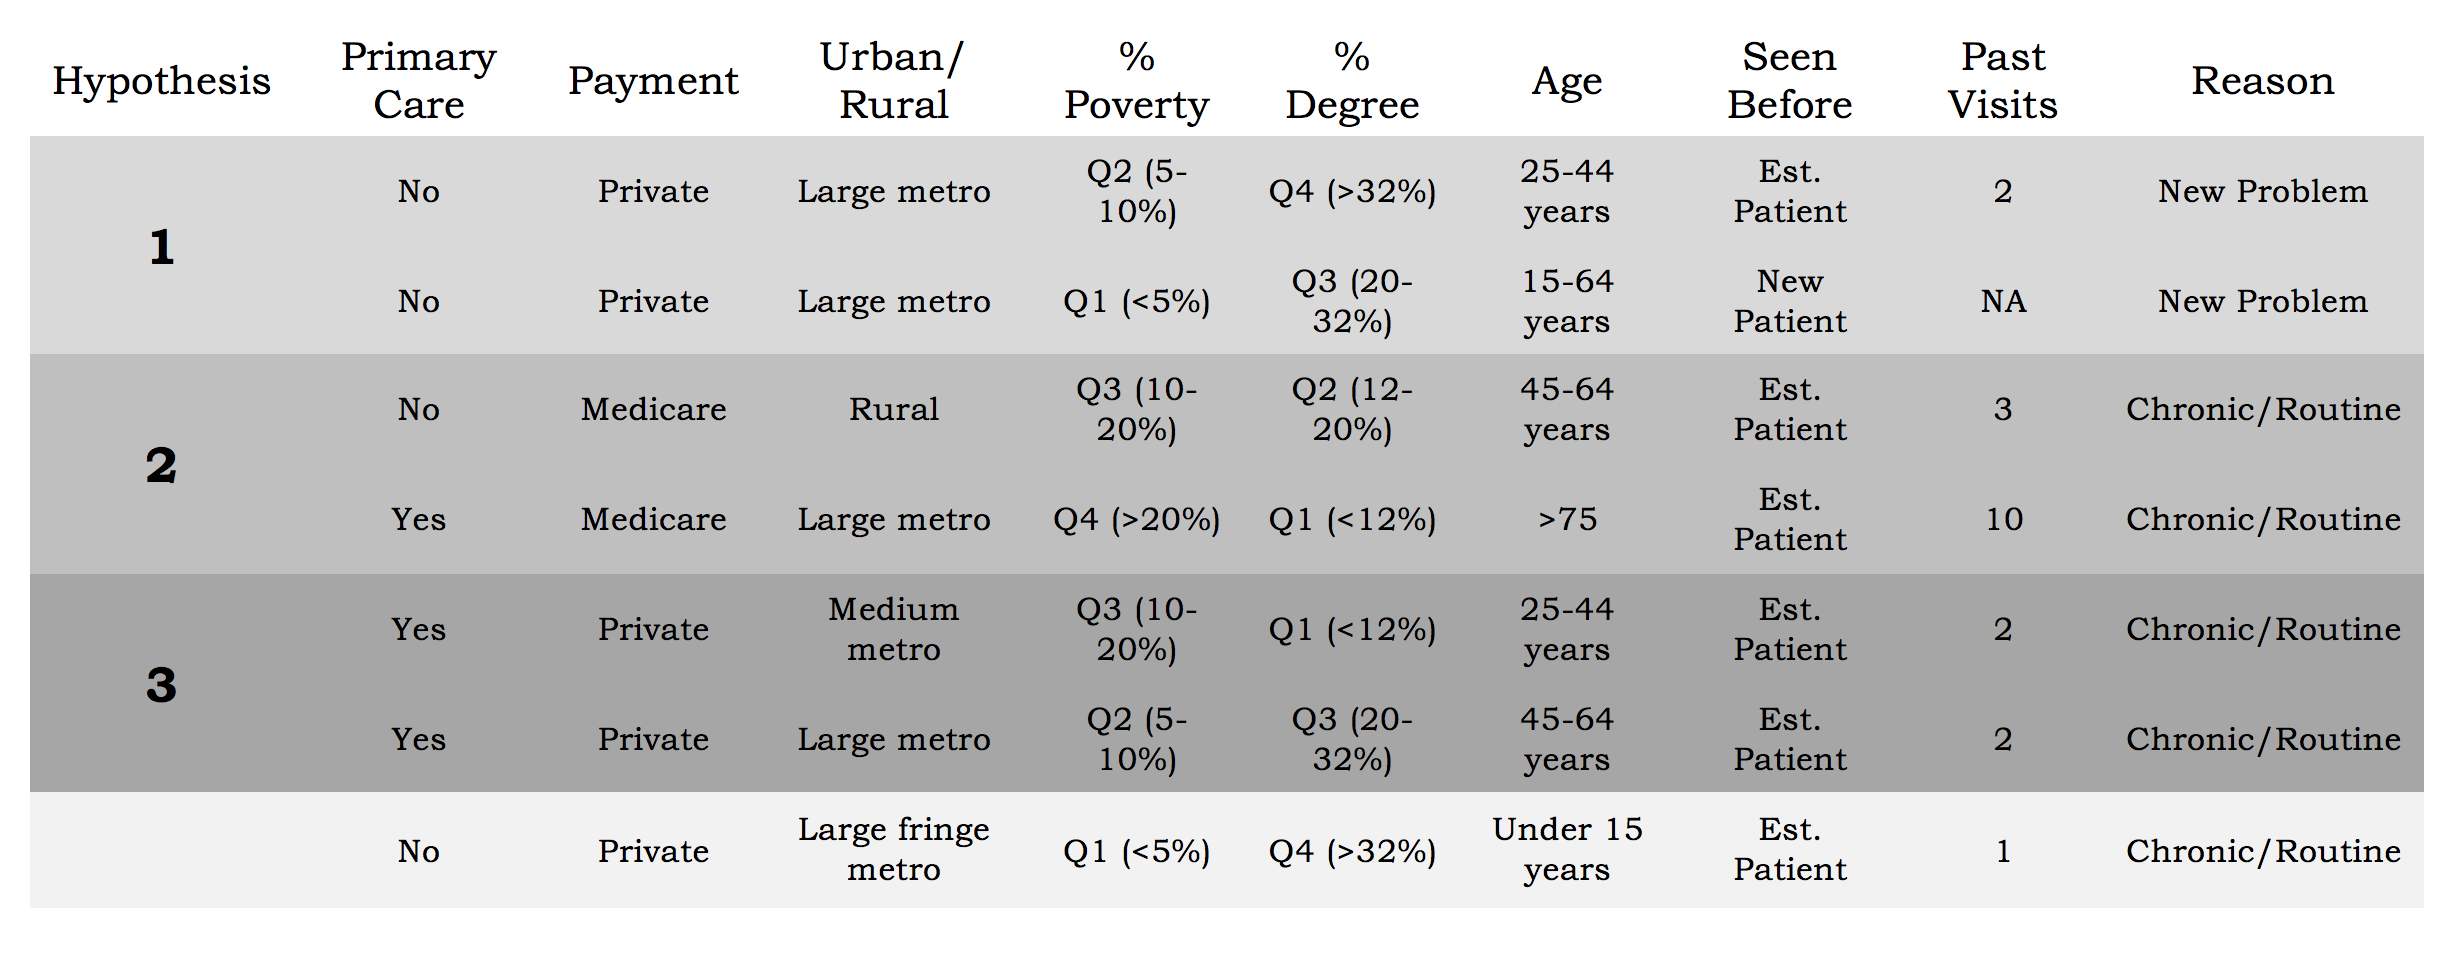
\includegraphics[scale = 0.45,angle = 90]{figures/clusters.png}
  \caption[Identified patient typologies of urgent care centers visits (2008-2012).]{\normalsize{Identified patient typologies of urgent care centers visits (2008-2012).}}
  \label{fig:clus1}
  \end{figure}
  
  \newpage
  
  Beginning with demographic trends, the characteristics which were
  \emph{not} identified as distinguishable in the sample by the clustering
  (and were thus not included in Table 1.) offer just as much, if not more
  insight as those that did result in fractioning. Race in particular was
  immediately noticeable for its lack of variety: of the initial clusters,
  all were predominantly or exclusively white, an unsurprising trend when
  one looks at the summary statistics (of the 3863 urgent care visits
  included in the data, 87\% of those were white individuals). This is
  substantively interesting for several reasons, mainly in that race is a
  known correlate with many other socioeconomic indicators, and urgent
  care appears to be largely utilized by white patients.
  
  Similarly, no significant clusters of patients going on weekends were
  identified, nor were any of the major clusters' visits injury related.
  These observations together seem to counter the typical view of urgent
  care, and coupled with the fact that only 25\% of the urgent care visits
  were coded as new visits, there are obvious indications that urgent care
  is being used in ways other than those proposed by hypothesis 1.
  
  Since the data set lacked individual level socioeconomic data, we can
  examine the socioeconomic indicators for the patients' ZIP codes which
  were included as demographic parameters proxies. Unsurprisingly, these
  appeared to cluster and correlate with both race and income: for both
  males and females, there were consistent clusters of White,
  25-44-year-old patients with private insurance, and both of these
  clusters were in the highest quartile of percent population with
  Bachelor's degrees, the second lowest percent population under the
  poverty line (5-10\%), and both visited clinics coded as being located
  in a ``Large central metro'' (Table 1.).
  
  In fact, if one predominant trend becomes clear from the demographic
  clustering, it is that urgent care centers are almost entirely an urban
  affair. Of the clusters found, all but one consisted of visits located
  in medium to large metros, indicating that while other variation between
  patients exists, most urgent care consumers are located in larger
  cities. And if its singularity wasn't enough, the cluster of visits
  which did occur in a rural setting also differed from most other
  clusters in the other parameters as well. As can be seen in the first
  row of Table 1., the rural cluster of visits had one of the highest
  levels of localized poverty, one of the lowest levels of educational
  attainment, and was one of only two clusters where a significant number
  of visits were paid with medicare.
  
  Also informative are the clusters' most occurring payment types, which
  complicate some of the theoretical notions of urgent care described in
  Chapter 1. While the largest clusters were consistently comprised of
  private insurance payers, Medicare without a doubt plays a role in
  getting people to urgent care centers. Medicare was listed as the
  primary payment method around 18 \% of the time, a large number when one
  considers the consumerist theories proposed in chapter one. These
  clusters are crucial to understanding the decision process behind
  choosing a health care provider, while simultaneously raising the
  question of the relationship between the surprising number of elderly
  patients on Medicare seeking treatment at an urgent care centers.
  
  The demographic characteristics of urgent care seekers were also
  clustered with behavioral, visit-level parameters in a second wave of
  cluster analysis, in order to to examine \emph{how} urgent care is
  utilized by different groups. By far the largest and most homogeneous
  clusters isolated consist of white, privately insured patients in medium
  to large urban environments. These trends match those found in the
  demographic clusters, and we can learn even more about this group by
  examining the cluster segmentation that occurred across their behavioral
  parameters in the second wave. Of the two clusters which consist almost
  entirely of white, 25-44-year-old men and women, both were almost
  entirely classed as ``established patients'', with at least one past
  visit. Also theoretically interesting, neither cluster had observations
  whose reason for visiting was ``injury related'' and neither had
  recorded visits on weekends. Clusters 5 and 6 in particular (Rows 5 and
  6, Table 1), consisted of 25-64-year-old white patients with private
  insurance, an established history of visiting urgent care, and a reason
  for their current visit coded as a ``chronic, routine problem''.
  
  In fact, only one cluster of visits in the final model were coded as new
  patients, though it is a sizable fraction of the whole.Ecxamining these
  two clusters reveals what I referred to earlier as the traditional
  patient characteristics ascribed to urgent care visits. These two
  cluster show what many would expect, both consisted of white, privately
  insured, new patients, and both clusters contain the only observations
  which occurred on a weekend or were coded as injury related. These
  characteristics are in line with what many hold as the purpose of urgent
  care centers, but they remain a small fraction of the recorded number of
  visits. Completely contradicting this idea, the other seven of the nine
  clusters identified have high levels of established patients with
  chronic or routine problems, with ages ranging for 15 to over 75.
  
  As for the Medicare question, if the clusters which consist of primarily
  elderly patients are examined, we can begin to understand a little
  better the relatively large percentage of what many would consider
  non-emergent care utilizers and their relationship to urgent care.
  Cluster 5 consists entirely of white patients over 74, whose visits were
  recorded as routine and who have a minimum of 3 past visits at the same
  center. Cluster three on the other hand has a slightly younger age
  range, and the majority of patients indicated that the urgent care
  center was \emph{not} their primary care. Also distinguishing, cluster
  three is the only cluster with a majority of rural observations. When
  compared, it appears that there are two typologies of elderly urgent
  care seekers, the first of which may be using urgent in much the same
  ways as the younger and larger clusters of privately insured urbanites,
  while the second seems to rely on urgent care much more as an actually
  resource for urgent problems.
  
  In the end, the observed typologies appear to correspond relatively well
  with all three hypotheses presented, with the exception of a relatively
  large number of very young urgent care goers who did not list it as
  their primary care physician. The explanation for this is probably as
  simple as them having a pediatrician, and using urgent care as a quick
  supplement, which somewhat supports hypothesis 3. What the cluster
  analysis really does is inform the analysis about which variables were
  identified as important to urgent care seekers. Using these, we can now
  turn to a logistic regression in order to understand better how each
  parameter influences decisions regarding urgent care
  
  \section{Testing Hypotheses}\label{testing-hypotheses}
  
  I test the hypotheses presented in the previous chapter using a series
  of logistic and multinomial logistic regressions. I find that while the
  data shows evidence for the first two theories, there is little evidence
  to support the theory that urgent care is being used solely as is often
  stated in the press. There appears to be clear significant indicators
  for individuals choosing to use urgent care as their primary care
  facility which follow the first hypothesis presented in the previous
  chapter. The data shows that for specific demographics, urgent care is a
  viable option for their primary care needs, adding evidence to the
  shifting tides of American primary care.
  
  \section*{Multinomial Logistic Regression
  Analysis}\label{multinomial-logistic-regression-analysis}
  \addcontentsline{toc}{section}{Multinomial Logistic Regression Analysis}
  
  The multinomial logistic regression tests the effect of our independant
  variables on four outcomes: 1) a visit to a traditional clinic whom the
  patient does \emph{not} identify as their primary care provider, 2) a
  visit to a traditional clinic whom the patient identifies as their
  primary care provider, 3) a visit to urgent care, not identified as the
  patient's primary care facility, and finally 4) a visit to urgent care
  where the patient identified the facility as their primary care
  provider.
  
  In order to understand the results of a multinomial logistic regression,
  it is important to keep in mind the reference group. Here, the group of
  patients who's visits occured at traditional practices, but who did not
  identify that practice as their primary care provider was used as the
  reference group. Thus, the three models show the effects for each of the
  idenpendant variables for the three other decisions in comparison to
  that initial reference point. The results of the regression are
  summarized in Table 5.4.
  
  \begin{verbatim}
  # weights:  28 (18 variable)
  initial  value 132022.357187 
  iter  10 value 79625.910851
  iter  20 value 77254.800517
  final  value 76960.219810 
  converged
  \end{verbatim}
  
  \begin{verbatim}
  # weights:  40 (27 variable)
  initial  value 132022.357187 
  iter  10 value 82725.013877
  iter  20 value 78584.252844
  iter  30 value 76292.877308
  iter  40 value 75778.907658
  iter  40 value 75778.906948
  iter  40 value 75778.906944
  final  value 75778.906944 
  converged
  \end{verbatim}
  
  \begin{verbatim}
  # weights:  32 (21 variable)
  initial  value 132022.357187 
  iter  10 value 82809.176942
  iter  20 value 74921.972136
  iter  30 value 71457.080672
  iter  40 value 71448.755860
  iter  40 value 71448.755399
  iter  40 value 71448.755396
  final  value 71448.755396 
  converged
  \end{verbatim}
  
  \begin{verbatim}
  # weights:  84 (60 variable)
  initial  value 132022.357187 
  iter  10 value 75711.213115
  iter  20 value 74293.011409
  iter  30 value 72092.532758
  iter  40 value 71167.815699
  iter  50 value 70298.559857
  iter  60 value 69977.828220
  iter  70 value 69899.813786
  final  value 69899.455337 
  converged
  \end{verbatim}
  
  \singlespacing
  
  \begin{table}
  \begin{center}
  \begin{footnotesize}
  \begin{tabular}{l c c c }
  \hline
   & Traditional Primary & Urgent Care & Urgent Care Primary \\
  \hline
  (Intercept)                  & $\mathbf{-0.36}^{***}$ & $\mathbf{-3.04}^{***}$ & $\mathbf{-4.07}^{***}$ \\
                               & $(0.02)$               & $(0.05)$               & $(0.09)$               \\
  `PCTPOVRHigh ZIP Poverty`    & $0.02$                 & $-0.05$                & $0.04$                 \\
                               & $(0.02)$               & $(0.07)$               & $(0.09)$               \\
  `HINCOMERHigh ZIP Income`    & $-0.06^{***}$          & $\mathbf{-0.38}^{***}$ & $\mathbf{-0.42}^{***}$ \\
                               & $(0.02)$               & $(0.06)$               & $(0.09)$               \\
  `PBAMORERHigh ZIP Education` & $\mathbf{-0.22}^{***}$ & $0.09$                 & $-0.08$                \\
                               & $(0.02)$               & $(0.06)$               & $(0.08)$               \\
  `URBANRURMedium Metro`       & $\mathbf{-0.19}^{***}$ & $\mathbf{0.29}^{***}$  & $0.31^{**}$            \\
                               & $(0.02)$               & $(0.06)$               & $(0.10)$               \\
  `URBANRURLarge Metro`        & $-0.08^{***}$          & $\mathbf{-0.43}^{***}$ & $0.29^{**}$            \\
                               & $(0.02)$               & $(0.07)$               & $(0.10)$               \\
  \hline
  AIC                          & 153956.44              & 153956.44              & 153956.44              \\
  BIC                          & 154126.79              & 154126.79              & 154126.79              \\
  Log\ Likelihood              & -76960.22              & -76960.22              & -76960.22              \\
  Deviance                     & 153920.44              & 153920.44              & 153920.44              \\
  Num.\ obs.                   & 95234                  & 95234                  & 95234                  \\
  \hline
  \multicolumn{4}{l}{\tiny{$^{***}p<0.001$, $^{**}p<0.01$, $^*p<0.05$}}
  \end{tabular}
  \end{footnotesize}
  \caption{Multinomial Logistic model: location effects}
  \label{table:coefficients}
  \end{center}
  \end{table}
  
  \begin{table}
  \begin{center}
  \begin{footnotesize}
  \begin{tabular}{l c c c }
  \hline
   & Traditional Primary & Urgent Care & Urgent Care Primary \\
  \hline
  (Intercept)              & $\mathbf{-0.44}^{***}$ & $\mathbf{-2.97}^{***}$ & $\mathbf{-4.17}^{***}$ \\
                           & $(0.02)$               & $(0.06)$               & $(0.09)$               \\
  AGE                      & $-0.00$                & $\mathbf{-0.01}^{***}$ & $0.00$                 \\
                           & $(0.00)$               & $(0.00)$               & $(0.00)$               \\
  SEXFemale                & $\mathbf{-0.06}^{***}$ & $-0.07$                & $0.12^{*}$             \\
                           & $(0.01)$               & $(0.04)$               & $(0.06)$               \\
  RACERBlack               & $\mathbf{0.21}^{***}$  & $-0.14$                & $\mathbf{0.40}^{***}$  \\
                           & $(0.02)$               & $(0.08)$               & $(0.09)$               \\
  RACEROther               & $\mathbf{0.19}^{***}$  & $-0.22$                & $0.21$                 \\
                           & $(0.03)$               & $(0.12)$               & $(0.14)$               \\
  PAYTYPERMedicaid         & $\mathbf{0.63}^{***}$  & $\mathbf{0.46}^{***}$  & $\mathbf{0.66}^{***}$  \\
                           & $(0.02)$               & $(0.07)$               & $(0.10)$               \\
  PAYTYPERMedicare         & $\mathbf{-0.53}^{***}$ & $0.13^{*}$             & $-0.10$                \\
                           & $(0.02)$               & $(0.06)$               & $(0.08)$               \\
  `PAYTYPERWorker's Comp`  & $\mathbf{-1.19}^{***}$ & $\mathbf{1.86}^{***}$  & $-0.05$                \\
                           & $(0.09)$               & $(0.09)$               & $(0.29)$               \\
  `PAYTYPERSelf-Pay/Other` & $\mathbf{-0.32}^{***}$ & $0.19^{*}$             & $0.33^{**}$            \\
                           & $(0.03)$               & $(0.07)$               & $(0.10)$               \\
  \hline
  AIC                      & 151611.81              & 151611.81              & 151611.81              \\
  BIC                      & 151867.34              & 151867.34              & 151867.34              \\
  Log\ Likelihood          & -75778.91              & -75778.91              & -75778.91              \\
  Deviance                 & 151557.81              & 151557.81              & 151557.81              \\
  Num.\ obs.               & 95234                  & 95234                  & 95234                  \\
  \hline
  \multicolumn{4}{l}{\tiny{$^{***}p<0.001$, $^{**}p<0.01$, $^*p<0.05$}}
  \end{tabular}
  \end{footnotesize}
  \caption{Multinomial Logistic model: demographic effects}
  \label{table:coefficients}
  \end{center}
  \end{table}
  
  \begin{table}
  \begin{center}
  \begin{footnotesize}
  \begin{tabular}{l c c c }
  \hline
   & Traditional Primary & Urgent Care & Urgent Care Primary \\
  \hline
  (Intercept)                        & $\mathbf{-1.55}^{***}$ & $\mathbf{-2.84}^{***}$ & $\mathbf{-5.00}^{***}$ \\
                                     & $(0.03)$               & $(0.05)$               & $(0.13)$               \\
  INJURYYes                          & $\mathbf{-0.49}^{***}$ & $\mathbf{0.54}^{***}$  & $-0.17$                \\
                                     & $(0.03)$               & $(0.06)$               & $(0.10)$               \\
  MAJORRoutine                       & $\mathbf{-0.61}^{***}$ & $\mathbf{-0.62}^{***}$ & $\mathbf{-0.90}^{***}$ \\
                                     & $(0.02)$               & $(0.06)$               & $(0.08)$               \\
  MAJORChronic                       & $\mathbf{-1.24}^{***}$ & $\mathbf{-0.36}^{***}$ & $\mathbf{-1.06}^{***}$ \\
                                     & $(0.02)$               & $(0.05)$               & $(0.07)$               \\
  `SENBEFORYes, established patient` & $\mathbf{1.64}^{***}$  & $\mathbf{-0.21}^{***}$ & $\mathbf{1.63}^{***}$  \\
                                     & $(0.03)$               & $(0.05)$               & $(0.14)$               \\
  PASTVIS                            & $\mathbf{0.01}^{***}$  & $-0.00$                & $\mathbf{0.01}^{***}$  \\
                                     & $(0.00)$               & $(0.00)$               & $(0.00)$               \\
  WEEKENDYES                         & $\mathbf{0.40}^{***}$  & $\mathbf{1.43}^{***}$  & $0.20$                 \\
                                     & $(0.07)$               & $(0.11)$               & $(0.27)$               \\
  \hline
  AIC                                & 142939.51              & 142939.51              & 142939.51              \\
  BIC                                & 143138.26              & 143138.26              & 143138.26              \\
  Log\ Likelihood                    & -71448.76              & -71448.76              & -71448.76              \\
  Deviance                           & 142897.51              & 142897.51              & 142897.51              \\
  Num.\ obs.                         & 95234                  & 95234                  & 95234                  \\
  \hline
  \multicolumn{4}{l}{\tiny{$^{***}p<0.001$, $^{**}p<0.01$, $^*p<0.05$}}
  \end{tabular}
  \end{footnotesize}
  \caption{Multinomial Logistic model: visit characteristics}
  \label{table:coefficients}
  \end{center}
  \end{table}
  
  \doublespacing
  
  \section*{Logistic Regression
  Analysis}\label{logistic-regression-analysis}
  \addcontentsline{toc}{section}{Logistic Regression Analysis}
  
  The initial exploratory analysis shows clear typologies of urgent care
  seekers which align with the hypotheses presented in the previous
  chapter, and the next phase of the analysis uses those trends and tests
  for significance using logistic regression analysis. Tables 5.1 and 5.2
  show the results of the two logistic regression models.
  
  \singlespacing
  
  \begin{table}
  \begin{center}
  \begin{footnotesize}
  \begin{tabular}{l c c c }
  \hline
   & Model 1 & Model 2 & Model 3 \\
  \hline
  Intercept                     & $-3.69^{***}$ & $-3.04^{***}$ & $-3.13^{***}$ \\
                                & $(0.06)$      & $(0.09)$      & $(0.11)$      \\
  Injury Related Visit          & $0.11^{*}$    &               & $-0.01$       \\
                                & $(0.04)$      &               & $(0.05)$      \\
  Weekend Visit                 & $0.06$        &               & $-0.10$       \\
                                & $(0.05)$      &               & $(0.07)$      \\
  Medicaid                      & $0.02$        &               & $-0.03$       \\
                                & $(0.03)$      &               & $(0.04)$      \\
  Medicare                      & $0.29^{***}$  &               & $0.26^{***}$  \\
                                & $(0.05)$      &               & $(0.05)$      \\
  SelfPay                       & $-0.34^{***}$ &               & $-0.36^{***}$ \\
                                & $(0.04)$      &               & $(0.04)$      \\
  Established Patient           & $0.06$        &               & $0.06$        \\
                                & $(0.04)$      &               & $(0.04)$      \\
  Number Past Visits            &               & $0.49^{***}$  & $0.48^{***}$  \\
                                &               & $(0.05)$      & $(0.05)$      \\
  Visit Reason: Preventative    &               & $0.99^{***}$  & $1.04^{***}$  \\
                                &               & $(0.10)$      & $(0.10)$      \\
  Visit Reason: Routine/Chronic &               & $-0.13^{*}$   & $-0.19^{**}$  \\
                                &               & $(0.06)$      & $(0.06)$      \\
  Age: Working                  &               & $0.10^{*}$    & $0.13^{*}$    \\
                                &               & $(0.04)$      & $(0.06)$      \\
  Age: Retired                  &               & $0.23^{***}$  & $0.21^{***}$  \\
                                &               & $(0.05)$      & $(0.05)$      \\
  Male                          &               & $-0.43^{***}$ & $-0.44^{***}$ \\
                                &               & $(0.08)$      & $(0.08)$      \\
  Race: White                   &               & $-0.00$       & $-0.00$       \\
                                &               & $(0.00)$      & $(0.00)$      \\
  High ZIP Income               &               & $-0.56^{***}$ & $-0.55^{***}$ \\
                                &               & $(0.06)$      & $(0.06)$      \\
  Rural                         &               & $-0.09^{*}$   & $-0.08^{*}$   \\
                                &               & $(0.04)$      & $(0.04)$      \\
  \hline
  AIC                           & 31001.63      & 30698.93      & 30588.75      \\
  BIC                           & 31069.06      & 30795.26      & 30742.88      \\
  Log Likelihood                & -15493.81     & -15339.47     & -15278.38     \\
  Deviance                      & 30987.63      & 30678.93      & 30556.75      \\
  Num. obs.                     & 112722        & 112722        & 112722        \\
  \hline
  \multicolumn{4}{l}{\tiny{$^{***}p<0.001$, $^{**}p<0.01$, $^*p<0.05$}}
  \end{tabular}
  \end{footnotesize}
  \caption{Logistic model of the decision to go to urgent care.}
  \label{table:coefficients}
  \end{center}
  \end{table}
  
  \begin{table}
  \begin{center}
  \begin{small}
  \begin{tabular}{l c c c }
  \hline
   & Model 1 & Model 2 & Model 3 \\
  \hline
  Intercept                     & $-0.06$       & $-4.58^{***}$ & $-3.62^{***}$ \\
                                & $(0.13)$      & $(0.25)$      & $(0.29)$      \\
  Injury Related Visit          & $-0.36^{***}$ &               & $-0.28^{*}$   \\
                                & $(0.10)$      &               & $(0.12)$      \\
  Weekend Visit                 & $-0.01$       &               & $0.05$        \\
                                & $(0.11)$      &               & $(0.17)$      \\
  Medicaid                      & $-0.30^{***}$ &               & $-0.16$       \\
                                & $(0.08)$      &               & $(0.09)$      \\
  Medicare                      & $-0.35^{**}$  &               & $-0.43^{***}$ \\
                                & $(0.11)$      &               & $(0.12)$      \\
  SelfPay                       & $-0.21^{*}$   &               & $-0.21^{*}$   \\
                                & $(0.09)$      &               & $(0.10)$      \\
  Established Patient           & $-0.95^{***}$ &               & $-0.94^{***}$ \\
                                & $(0.10)$      &               & $(0.11)$      \\
  Number Past Visits            &               & $-0.63^{***}$ & $-0.50^{***}$ \\
                                &               & $(0.13)$      & $(0.13)$      \\
  Visit Reason: Preventative    &               & $-1.02^{**}$  & $-1.12^{***}$ \\
                                &               & $(0.32)$      & $(0.33)$      \\
  Visit Reason: Routine/Chronic &               & $3.69^{***}$  & $3.63^{***}$  \\
                                &               & $(0.22)$      & $(0.23)$      \\
  Age: Working                  &               & $0.02^{***}$  & $0.02^{***}$  \\
                                &               & $(0.00)$      & $(0.00)$      \\
  Age: Retired                  &               & $1.04^{***}$  & $1.10^{***}$  \\
                                &               & $(0.13)$      & $(0.14)$      \\
  Male                          &               & $-0.32^{***}$ & $-0.31^{**}$  \\
                                &               & $(0.09)$      & $(0.09)$      \\
  Race: White                   &               &               & $-0.03$       \\
                                &               &               & $(0.14)$      \\
  High ZIP Income               &               &               & $-0.20$       \\
                                &               &               & $(0.15)$      \\
  Rural                         &               &               & $-0.25$       \\
                                &               &               & $(0.14)$      \\
  \hline
  AIC                           & 4027.38       & 3611.24       & 3507.18       \\
  BIC                           & 4070.48       & 3654.34       & 3605.69       \\
  Log Likelihood                & -2006.69      & -1798.62      & -1737.59      \\
  Deviance                      & 4013.38       & 3597.24       & 3475.18       \\
  Num. obs.                     & 3488          & 3488          & 3488          \\
  \hline
  \multicolumn{4}{l}{\tiny{$^{***}p<0.001$, $^{**}p<0.01$, $^*p<0.05$}}
  \end{tabular}
  \end{small}
  \caption{Logistic model of the decision to use urgent care as primary care}
  \label{table:coefficients}
  \end{center}
  \end{table}
  
  \doublespacing
  
  The first table is a model of the initial decision to go to urgent care.
  For the odds of choosing to go to urgent care over other means of
  ambulatory care, there is no significance for whether or not the visit
  is injury related, and whether or not it is a weekend. This supports the
  observations from the cluster analysis, and provides further evidence
  against the demand oriented hypothesis. Similarly, visits for routine
  and chronic issues have a higher chance of leading to an urgent care
  visit than problems less than 3 mos old. These trends both support
  Hypothesis 3: that urgent care centers are being used as a new mode of
  primary care.
  
  For the second analysis, the outcome is no longer whether or not the
  visit was \emph{at} urgent care, but whether or not an urgent care
  patient listed the urgent care center as their ``Primary Health
  Provider''. Interestingly, most of the significant variables' effects
  change direction when this is taken as the outcome. While high local
  income levels had a negative relationship with the decision to go to
  urgent care, it appears to very positively correlate with those who do
  use urgent care as their primary care.
  
  Many of the visit-specific variables that did not have a significant
  effect on the odds of choosing urgent care became significant when
  looking at urgent care as primary care. Unsurprisingly, whether or not
  the visit was injury related has a negative effect on the odds of the
  patient specifying that clinic as their primary care.
  
  There are some surprising trends in the secondary logistic model which
  deserve further study. Established patient, for example, have a
  significant negative correlation with the odds of a patient using urgent
  care as their primary care physician, as did number of past visits. A
  further look into the structure of the data reveals a plausible
  explanation: while 94\% of patients who listed the urgent care center as
  their primary care physician were recorded as Established patients, this
  group as a whole only constitutes a third of the total number of visits
  to urgent care. In other words, there were two-thirds as many urgent
  care visits who were established patients, yet did \emph{not} list the
  facility as their primary care office, and this trend is similar for
  number of past visits.
  
  \section*{Revisiting the hypotheses}\label{revisiting-the-hypotheses}
  \addcontentsline{toc}{section}{Revisiting the hypotheses}
  
  \doublespacing
  Returning to the theoretical explanations for urgent care, it appears
  that while no one theory explains the totality of urgent care center
  usage, I observed much more evidence for hypotheses 1 and 3 than for
  2---unsuprising given that the theory behind hypothesis two is the one
  most often cited in popular press stories about urgent care. There seems
  to be plenty of observable evidence to support hypothesis 3: there were
  a number of clusters which not only corresponded to the predicted trends
  for that hypothesis, but which directly stated that they use urgent care
  as their primary care provider.
  
  \chapter*{Conclusion}\label{conclusion}
  \addcontentsline{toc}{chapter}{Conclusion}
  
  \setcounter{chapter}{6} \setcounter{section}{0} \doublespacing
  
  In this thesis, I have attempted to examine the relatively new
  phenomenon of urgent care centers and their use patterns, reviewing
  where the sociology of medicine has been and where the American health
  care system is now. While the analysis was limited by the data
  availability, the observed groupings of urgent care patients and the
  significant factors for the decision to use it as urgent care allow us
  to begin to answer questions about who's going to urgent care and their
  reasoning.
  
  With the rapidly increasing amount of data, further research into urgent
  care centers could benefit from a times series study, in order to answer
  some of the questions raised about whether or not patient behavior is
  changing or just dispersing. Additionally, there are an increasing
  number of health care practices which resemble urgent care, retail
  clinics located inside large stores being just one example, that could
  shed further light on the modern patient as a health consumer.
  
  \chapter*{Appendix A}\label{appendix-a}
  \addcontentsline{toc}{chapter}{Appendix A}
  
  \newpage
  
  \doublespacing
  
  \singlespacing
  
  \begin{longtable}[c]{@{}lll@{}}
  \caption{Observed Proportions of Independant Variables
  \label{tab:sums}}\tabularnewline
  \toprule
  Variable & Category & Percentage\tabularnewline
  \midrule
  \endfirsthead
  \toprule
  Variable & Category & Percentage\tabularnewline
  \midrule
  \endhead
  Sex & &\tabularnewline
  & Female & 57.1\tabularnewline
  & Male & 42.9\tabularnewline
  AgeGroup & &\tabularnewline
  & 15-24 years & 8.68\tabularnewline
  & 25-44 years & 22.89\tabularnewline
  & 45-64 years & 29.63\tabularnewline
  & 65-74 years & 13.93\tabularnewline
  & 75 years and over & 12.58\tabularnewline
  & Under 15 years & 12.3\tabularnewline
  Race & &\tabularnewline
  & Black & 9.15\tabularnewline
  & Other & 3.87\tabularnewline
  & White & 86.98\tabularnewline
  PaymentType & &\tabularnewline
  & All sources of payment are blank & 0.44\tabularnewline
  & Medicaid & 10.67\tabularnewline
  & Medicare & 26.37\tabularnewline
  & No charge & 0.58\tabularnewline
  & Other & 3.07\tabularnewline
  & Private insurance & 46.9\tabularnewline
  & Self-pay & 4.86\tabularnewline
  & Unknown & 1.93\tabularnewline
  & Worker's compensation & 5.17\tabularnewline
  UrbanCategory & &\tabularnewline
  & Large central metro & 24.6\tabularnewline
  & Large fringe metro & 14.62\tabularnewline
  & Medium metro & 34.55\tabularnewline
  & Micropolitan/noncore (nonmetro) & 15.98\tabularnewline
  & Missing data & 0\tabularnewline
  & Small metro & 10.25\tabularnewline
  PercentPoverty & &\tabularnewline
  & Missing data & 0\tabularnewline
  & Quartile 1 (Less than 5.00 percent) & 18.16\tabularnewline
  & Quartile 2 (5.00-9.99 percent) & 30.24\tabularnewline
  & Quartile 3 (10.00-19.99 percent) & 39.22\tabularnewline
  & Quartile 4 (20.00 percent or more) & 12.38\tabularnewline
  \bottomrule
  \end{longtable}
  
  \chapter*{Appendix B}\label{appendix-b}
  \addcontentsline{toc}{chapter}{Appendix B}
  
  \doublespacing
  
  \subsubsection*{K-modes / Why cluster?}\label{k-modes-why-cluster}
  \addcontentsline{toc}{subsubsection}{K-modes / Why cluster?}
  
  In the supervised learning world, the data in question has an obvious
  response variable, which is tested against a null hypothesis based on
  theory. For this case, we do not know exactly what the outcome of
  interest is for those patients who went to urgent care, rather we are
  interested in the characteristics of who is choosing to go there. For
  such a data set, clustering methods allow us to examine the data in an
  \emph{unsupervised} manner --- mainly in that we let the statistical
  software find the patterns rather than test for patterns at the start.
  
  \subsubsection*{Methodological
  Considerations}\label{methodological-considerations}
  \addcontentsline{toc}{subsubsection}{Methodological Considerations}
  
  To perform the analysis on the data, four key methodological decisions
  were made by following either statistical convention or similar previous
  anlayses. All variables were re-coded as dummy variables, and the
  distances between these were standardized on a scale from 0 to 1, so as
  to prevent any skewdness which might result. Second, I chose to use the
  measure of distance known as the Jaccard method, which is specifically
  created to measure the distance between 0 to 1 scaled variables. It also
  has the unique feature of not including as significant pairs which both
  have 0 for a parameter. This is substantively important since though two
  visits may both have 0's for Private Insurance for example, the fact
  that they both don't have private insurance is not enough to consider
  them theoretically simliar by negation: one may be on medicare while the
  other may be uninsured. Third, for the actual groupings themselves, I
  have chosen the standard Ward's method, which attempts to minimize the
  variance within groups and thus maximizes the homogenaity. Fourth, in
  keeping with similar exploratory anlyses, I have limited the clusters to
  a theoretically interesting number while keeping a managable
  representation of reality.
  
  \subsubsection*{Determining the number of
  Clusters}\label{determining-the-number-of-clusters}
  \addcontentsline{toc}{subsubsection}{Determining the number of Clusters}
  
  Because urgent care centers have been greatly ignored by sociologists
  studying medical practices, there was little theoretical guidance in
  selecting a likely number of subgroups for the analysis. Similarly,
  because I am interested in understanding how an unsupervised analysis of
  patient data will reveal trends, it was particuarly important to the
  analysis that the number of clusters were both methematically acheivable
  and substantivly small enough for analysis.
  
  To accomplish this, I began with hierarchal clustering of the random
  samples chosen from the data. Using a mixed-methods tool to calculate
  the distance matrix between the various observations, I placed each
  point into an althgorithm which subsequently minimized the variance
  between clusters. Figure 1 shows the banner graph for the initial
  agglomerative cluster methods for the behavioral variables.
  
  \begin{figure}[htbp]
  \centering
  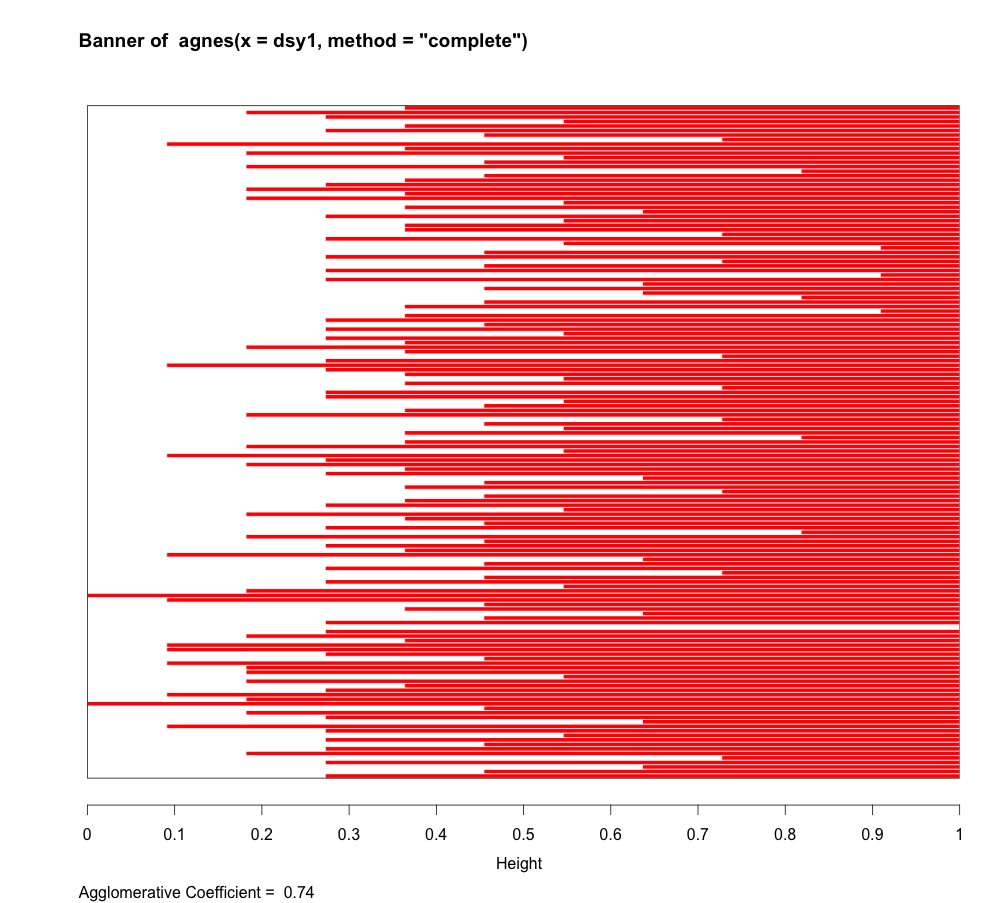
\includegraphics[scale = 0.35,angle = 0]{figures/banner.png}
  \caption[Sample Banner Agglomerative Clustering Results]{\normalsize{Sample Banner Agglomerative Clustering Results}}
  \label{fig:ban1}
  \end{figure}
  
  The white lines extending to the right represent clusters which differ
  from each other. After running the bottom up clustering method for a
  number of trials, the agglomerative coefficient was always between .73
  and .8, indicating that as the height for which the clusters should stop
  combining. Again, Figure 1 demonstrates that at that height, around 8
  clusters are have clearly seperated.
  
  \subsubsection*{OR}\label{or}
  \addcontentsline{toc}{subsubsection}{OR}
  
  Because urgent care centers have been significantly overlooked by
  sociologists studying medical practices, there was little theoretical
  guidance in selecting a likely number of subgroups for the cluster
  analysis, often the first step in such examinations. Similarly, because
  I am interested in understanding how an unsupervised analysis of patient
  data will reveal trends, rather than imposing them onto the data, it was
  particularly important to the investigation that the number of clusters
  be both mathematically achievable and substantively small enough for
  analysis while still remaining unsupervised. The general rule of thumb
  for cluster analysis suggested by Mardia, Kent and Bibbby (1997)
  stipulates that the number of clusters k is approximately the square
  root of n / 2. However, in the case of our comparably small sample of
  urgent care visitors recorded in the NAMCS data set, such a rule would
  indicate at least 30 clusters---clearly not a workable number to make
  sense of patterns in urgent care patients and their use.
  
  Instead, to estimate a k which would produce heterogeneous groups while
  still remaining theoretically enlightening, I began with non-guided
  hierarchal clustering of samples of 200 visits to urgent care centers
  randomly chosen from the data. Using the Gower methodology of finding
  the distance between dissimilar variable types, I calculated the
  distance matrix between the various observations for each sample. These
  distance measures were then used as the input to a hierarchal clustering
  algorithm which attempted to minimize the distance between observations
  within the same groups while maximizing the distance between them.
  Figure 1 shows the `banner' for the initial agglomerative cluster
  methods for the behavioral variables, and can be understood as a
  graphical representation of the points at which a cluster breaks away
  from the pack of observations. The white lines extending to the right
  represent clusters at their separation point, where larger red areas
  between white lines indicate stronger outside group variance.
  
  It should be noted that though the analyses were performed in two waves,
  the clusters should be examined with each other in mind, and I have
  included some of the key demographic variables in with the behavioral
  variables to that end. {[}OH YEAH, THIS IS GOING IN THE APPENDIX{]}
  
  \emph{Figure 2. Color coded clusters.}
  
  Figure 1 above shows the typical spread of the behavioral parameters'
  clusters, and is useful for keeping the proportions of clusters in mind.
  
  \backmatter
  
  \chapter*{Bibliography}\label{bibliography}
  \addcontentsline{toc}{chapter}{Bibliography}
  
  \noindent
  \setlength{\parindent}{-0.20in} \setlength{\leftskip}{0.20in}
  \setlength{\parskip}{8pt}
  
  \hypertarget{refs}{}
  \hypertarget{ref-ACPux5fimpendingux5f2006}{}
  , ACP. 2006. \emph{The Impending Collapse of Primary Care Medicine and
  Its Implications for the State of the Nation's Health Care}. American
  College of Physicians. Retrieved April 15, 2016
  (\url{http://www.providersedge.com/ehdocs/ehr_articles/The_Impending_Collapse_of_Primary_Care_Medicine_and_Its_Implications_for_the_State_of_the_Nation-s_Healthcare.pdf}).
  
  \hypertarget{ref-CONSUMERux5fHEALTH}{}
  Anon. n.d. ``A Study of Consumer Attitudes About Health Care: The Role
  of the Emergency Room on JSTOR.'' Retrieved September 21, 2015a
  (\url{http://www.jstor.org/stable/3763675}).
  
  \hypertarget{ref-manyux5fER}{}
  Anon. n.d. ``Many Emergency Department Visits Could Be Managed At Urgent
  Care Centers And Retail Clinics - ProQuest.'' Retrieved September 21,
  2015b
  (\url{http://search.proquest.com/docview/755047690/TextGraphic/1?accountid=13475}).
  
  \hypertarget{ref-namcs}{}
  Anon. n.d. ``NAMCS/NHAMCS - Questionnaires, Datasets, and Related
  Documentation.'' Retrieved March 4, 2016c
  (\url{http://www.cdc.gov/nchs/ahcd/ahcd_questionnaires.htm\#documentation}).
  
  \hypertarget{ref-UCux5fMarket}{}
  Anon. n.d. ``Urgent Care Centers in the US Market Research IBISWorld.''
  Retrieved September 16, 2015d
  (\url{http://www.ibisworld.com/industry/urgent-care-centers.html}).
  
  \hypertarget{ref-barkerux5felectronicux5f2008}{}
  Barker, Kristin K. 2008. ``Electronic Support Groups, Patient-Consumers,
  and Medicalization: The Case of Contested Illness.'' \emph{Journal of
  Health and Social Behavior} 49(1):20--36. Retrieved November 24, 2015
  (\url{http://www.jstor.org/stable/27638733}).
  
  \hypertarget{ref-UCux5f10STATS}{}
  Becker. n.d. ``10 Statistics on Urgent Care Centers.'' Retrieved
  September 21, 2015
  (\url{http://www.beckershospitalreview.com/hospital-management-administration/10-statistics-on-urgent-care-centers.html}).
  
  \hypertarget{ref-bloomux5fdoctorux5f1965}{}
  Bloom, Samuel William. 1965. \emph{The Doctor and His Patient.}
  Collier-Macmillan: Free Press ;
  
  \hypertarget{ref-boyerux5fexaminingux5f2010}{}
  Boyer, Carol A. and Karen E. Lutfey. 2010. ``Examining Critical Health
  Policy Issues Within and Beyond the Clinical Encounter:
  Patient---Provider Relationships and Help-Seeking Behaviors.''
  \emph{Journal of Health and Social Behavior} 51:S80--S93. Retrieved
  November 24, 2015 (\url{http://www.jstor.org/stable/20798318}).
  
  \hypertarget{ref-HEALTHux5fTRACKINGux5f2012}{}
  Center for Studying Health System Change. 2012. \emph{Health Tracking
  Household Survey, 2010 {[}United States{]}: Version 1}. Retrieved
  September 15, 2015
  (\url{http://www.icpsr.umich.edu/HMCA/studies/34141/version/1}).
  
  \hypertarget{ref-draperux5fprimary-careux5f1975}{}
  Draper, Peter and Helen L. Smits. 1975. ``The Primary-Care Practitioner
  --- Specialist or Jack-of-All-Trades.'' \emph{New England Journal of
  Medicine} 293(18):903--7. Retrieved November 24, 2015
  (\url{http://www.nejm.org/doi/abs/10.1056/NEJM197510302931805}).
  
  \hypertarget{ref-egbertux5freductionux5f1964}{}
  Egbert, Lawrence D., George E. Battit, Claude E. Welch, and Marshall K.
  Bartlett. 1964. ``Reduction of Postoperative Pain by Encouragement and
  Instruction of Patients: A Study of Doctor-Patient Rapport.'' \emph{New
  England Journal of Medicine} 270(16):825--27. Retrieved November 24,
  2015 (\url{http://www.nejm.org/doi/abs/10.1056/NEJM196404162701606}).
  
  \hypertarget{ref-freidsonux5fsociologyux5f1961}{}
  Freidson, Eliot. 1961. ``The Sociology of Medicine.'' \emph{Current
  Sociology} 10(3):123--40. Retrieved April 15, 2016
  (\url{http://csi.sagepub.com/content/10/3/123}).
  
  \hypertarget{ref-grayux5ftrustux5f1997}{}
  Gray, B. H. 1997. ``Trust and Trustworthy Care in the Managed Care
  Era.'' \emph{Health Affairs} 16(1):34--49. Retrieved April 15, 2016
  (\url{http://content.healthaffairs.org/content/16/1/34}).
  
  \hypertarget{ref-HCUP}{}
  HCUP. n.d. ``HCUP Fast Stats.'' Retrieved September 15, 2015
  (\url{http://www.hcup-us.ahrq.gov/faststats/StatePayerServlet?state1=OR}).
  
  \hypertarget{ref-heritageux5fproblemsux5f2006}{}
  Heritage, John and Douglas W. Maynard. 2006. ``Problems and Prospects in
  the Study of Physician-Patient Interaction: 30 Years of Research.''
  \emph{Annual Review of Sociology} 32:351--74. Retrieved November 24,
  2015 (\url{http://www.jstor.org/stable/29737743}).
  
  \hypertarget{ref-hibbardux5fconsumerismux5f1987}{}
  Hibbard, Judith H. and Edward C. Weeks. 1987. ``Consumerism in Health
  Care: Prevalence and Predictors.'' \emph{Medical Care} 25(11):1019--32.
  Retrieved April 15, 2016 (\url{http://www.jstor.org/stable/3765391}).
  
  \hypertarget{ref-kabaux5fevolutionux5f2007}{}
  Kaba, R. and P. Sooriakumaran. 2007. ``The Evolution of the
  Doctor-Patient Relationship.'' \emph{International Journal of Surgery}
  5(1):57--65. Retrieved November 24, 2015
  (\url{http://www.sciencedirect.com/science/article/pii/S1743919106000094}).
  
  \hypertarget{ref-lamontux5fstudyux5f2002}{}
  Lamont, Michèle and Virág Molnár. 2002. ``The Study of Boundaries in the
  Social Sciences.'' \emph{Annual Review of Sociology} 28:167--95.
  Retrieved November 24, 2015 (\url{http://www.jstor.org/stable/3069239}).
  
  \hypertarget{ref-lawsux5femergenceux5f2008}{}
  Laws, Margaret and Mary Kate Scott. 2008. ``The Emergence Of
  Retail-Based Clinics In The United States: Early Observations.''
  \emph{Health Affairs} 27(5):1293--8. Retrieved November 24, 2015
  (\url{http://content.healthaffairs.org/content/27/5/1293}).
  
  \hypertarget{ref-luptonux5fconsumerismux5f1997}{}
  Lupton, Deborah. 1997. ``Consumerism, Reflexivity and the Medical
  Encounter.'' \emph{Social Science \& Medicine} 45(3):373--81. Retrieved
  November 24, 2015
  (\url{http://www.sciencedirect.com/science/article/pii/S027795369600353X}).
  
  \hypertarget{ref-luptonux5fcaveatux5f1991}{}
  Lupton, Deborah, Cam Donaldson, and Peter Lloyd. 1991. ``Caveat Emptor
  or Blissful Ignorance? Patients and the Consumerist Ethos.''
  \emph{Social Science \& Medicine} 33(5):559--68. Retrieved November 24,
  2015
  (\url{http://www.sciencedirect.com/science/article/pii/027795369190213V}).
  
  \hypertarget{ref-mayux5fclinicalux5f2007}{}
  May, Carl. 2007. ``The Clinical Encounter and the Problem of Context.''
  \emph{Sociology} 41(1):29--45. Retrieved November 24, 2015
  (\url{http://soc.sagepub.com/content/41/1/29}).
  
  \hypertarget{ref-mckinlayux5fendux5f2002}{}
  McKinlay, John B. and Lisa D. Marceau. 2002. ``The End of the Golden Age
  of Doctoring.'' \emph{International Journal of Health Services}
  32(2):379--416. Retrieved April 15, 2016
  (\url{http://joh.sagepub.com/content/32/2/379}).
  
  \hypertarget{ref-mechanicux5fsociologyux5f1966}{}
  Mechanic, David. 1966. ``The Sociology of Medicine: Viewpoints and
  Perspectives.'' \emph{Journal of Health and Human Behavior} 7(4):237.
  Retrieved November 24, 2015
  (\url{http://www.jstor.org/stable/2948770?origin=crossref}).
  
  \hypertarget{ref-mehrotraux5fretailux5f2008}{}
  Mehrotra, Ateev, Margaret C. Wang, Judith R. Lave, John L. Adams, and
  Elizabeth A. McGlynn. 2008. ``Retail Clinics, Primary Care Physicians,
  And Emergency Departments: A Comparison Of Patients' Visits.''
  \emph{Health Affairs} 27(5):1272--82. Retrieved September 21, 2015
  (\url{http://content.healthaffairs.org/content/27/5/1272}).
  
  \hypertarget{ref-millerux5fprimaryux5f2010}{}
  Miller, William L., Benjamin F. Crabtree, Paul A. Nutting, Kurt C.
  Stange, and Carlos Roberto Jaén. 2010. ``Primary Care Practice
  Development: A Relationship-Centered Approach.'' \emph{The Annals of
  Family Medicine} 8(Suppl 1):S68--S79. Retrieved November 24, 2015
  (\url{http://www.annfammed.org/content/8/Suppl_1/S68}).
  
  \hypertarget{ref-OMALLEYux5f2013}{}
  O'Malley, Ann S. 2013. ``After-Hours Access To Primary Care Practices
  Linked With Lower Emergency Department Use And Less Unmet Medical
  Need.'' \emph{Health Affairs} 32(1):175--83. Retrieved September 15,
  2015 (\url{http://content.healthaffairs.org/content/32/1/175}).
  
  \hypertarget{ref-petersenux5fnonurgentux5f1998}{}
  Petersen, L. A., H. R. Burstin, A. C. O'Neil, E. J. Orav, and T. A.
  Brennan. 1998. ``Nonurgent Emergency Department Visits - The Effect of
  Having a Regular Doctor.'' \emph{Medical Care} 36(8):1249--55.
  
  \hypertarget{ref-phillipsux5fprimaryux5f2010}{}
  Phillips, Robert L. and Andrew W. Bazemore. 2010. ``Primary Care And Why
  It Matters For U.S. Health System Reform.'' \emph{Health Affairs}
  29(5):806--10. Retrieved November 24, 2015
  (\url{http://content.healthaffairs.org/content/29/5/806}).
  
  \hypertarget{ref-pittsux5fwhereux5f2010}{}
  Pitts, Stephen R., Emily R. Carrier, Eugene C. Rich, and Arthur L.
  Kellermann. 2010. ``Where Americans Get Acute Care: Increasingly, It's
  Not At Their Doctor's Office.'' \emph{Health Affairs} 29(9):1620--9.
  Retrieved September 21, 2015
  (\url{http://content.healthaffairs.org/content/29/9/1620}).
  
  \hypertarget{ref-potterux5frelationshipux5f2005}{}
  Potter, Sharyn J. and John B. McKinlay. 2005. ``From a Relationship to
  Encounter: An Examination of Longitudinal and Lateral Dimensions in the
  Doctor-Patient Relationship.'' \emph{Social Science \& Medicine (1982)}
  61(2):465--79.
  
  \hypertarget{ref-reederux5fpatient-clientux5f1972}{}
  Reeder, Leo G. 1972. ``The Patient-Client as a Consumer: Some
  Observations on the Changing Professional-Client Relationship.''
  \emph{Journal of Health and Social Behavior} 13(4):406--12. Retrieved
  November 24, 2015 (\url{http://www.jstor.org/stable/2136833}).
  
  \hypertarget{ref-reichux5fcontradictionsux5f2014}{}
  Reich, Adam D. 2014. ``Contradictions in the Commodification of Hospital
  Care.'' \emph{American Journal of Sociology} 119(6):1576--1628.
  Retrieved November 24, 2015
  (\url{http://www.jstor.org/stable/10.1086/676836}).
  
  \hypertarget{ref-rubinux5furgentux5f2012}{}
  Rubin, Mike. 2012. ``Urgent Care.'' \emph{EMS World} 41(4):70. Retrieved
  September 21, 2015
  (\url{http://search.proquest.com/docview/1007867084/abstract?}).
  
  \hypertarget{ref-shawux5f2013}{}
  Shaw, Eric K. et al. 2013. ``Decision-Making Processes of Patients Who
  Use the Emergency Department for Primary Care Needs.'' \emph{Journal of
  Health Care for the Poor and Underserved} 24(3):1288--1305. Retrieved
  September 21, 2015
  (\url{https://muse.jhu.edu/journals/journal_of_health_care_for_the_poor_and_underserved/v024/24.3.shaw.html}).
  
  \hypertarget{ref-SHORTLIFFEux5f1958}{}
  Shortliffe, Ernest C., T. Stewart Hamilton, and Edward H. Noroian. 1958.
  ``The Emergency Room and the Changing Pattern of Medical Care.''
  \emph{New England Journal of Medicine} 258(1):20--25. Retrieved
  September 15, 2015
  (\url{http://dx.doi.org/10.1056/NEJM195801022580105}).
  
  \hypertarget{ref-southertonux5fboundariesux5f2002}{}
  Southerton, Dale. 2002. ``Boundaries of `Us' and `Them': Class, Mobility
  and Identification in a New Town.'' \emph{Sociology} 36(1):171--93.
  Retrieved November 24, 2015
  (\url{http://soc.sagepub.com/content/36/1/171}).
  
  \hypertarget{ref-starrux5fsocialux5f1982}{}
  Starr, Paul. 1982. \emph{The Social Transformation of American
  Medicine}. Basic Books.
  
  \hypertarget{ref-timmermansux5fcontinuedux5f2010}{}
  Timmermans, Stefan and Hyeyoung Oh. 2010. ``The Continued Social
  Transformation of the Medical Profession.'' \emph{Journal of Health and
  Social Behavior} 51:S94--S106. Retrieved November 24, 2015
  (\url{http://www.jstor.org/stable/20798319}).
  
  \hypertarget{ref-ullmanux5fPATIENTS}{}
  Ullman, Ralph, James Block, and William C. Stratmann. n.d. ``An
  Emergency Room's Patients: Their Characteristics and Utilization of
  Hospital Services on JSTOR.'' Retrieved September 21, 2015
  (\url{http://www.jstor.org/stable/3763673}).
  
  \hypertarget{ref-wangux5fwhyux5f2010}{}
  Wang, Margaret C., Gery Ryan, Elizabeth A. McGlynn, and Ateev Mehrotra.
  2010. ``Why Do Patients Seek Care at Retail Clinics, and What
  Alternatives Did They Consider?'' \emph{American Journal of Medical
  Quality} 25(2):128--34. Retrieved September 21, 2015
  (\url{http://ajm.sagepub.com/content/25/2/128}).
  
  \hypertarget{ref-WEINECKux5fNOAPPT}{}
  Weinick, Robin M. and Renée M. Betancourt. n.d. ``No Appointment Needed:
  The Resurgence of Urgent Care Centers in the United States.''
  
  \hypertarget{ref-WEINECKux5f2009}{}
  Weinick, Robin M., Steffanie J. Bristol, and Catherine M. DesRoches.
  2009. ``Urgent Care Centers in the U.S.: Findings from a National
  Survey.'' \emph{BMC Health Services Research} 9:79. Retrieved September
  21, 2015 (\url{http://www.ncbi.nlm.nih.gov/pmc/articles/PMC2685126/}).
  
  \hypertarget{ref-weinickux5furgentux5f2009-1}{}
  Weinick, Robin M., Steffanie J. Bristol, and Catherine M. DesRoches.
  2009. ``Urgent Care Centers in the U.S.: Findings from a National
  Survey.'' \emph{BMC Health Services Research} 9(1):79. Retrieved
  November 24, 2015
  (\url{http://www.biomedcentral.com/1472-6963/9/79/abstract}).
  
  \hypertarget{ref-wrightux5fmedicalux5f2010}{}
  Wright, Eric R. and Brea L. Perry. 2010. ``Medical Sociology and Health
  Services Research: Past Accomplishments and Future Policy Challenges.''
  \emph{Journal of Health and Social Behavior} 51:S107--S119. Retrieved
  November 24, 2015 (\url{http://www.jstor.org/stable/20798320}).
  
  \hypertarget{ref-yeeux5fsurgeux5f2013}{}
  Yee, Tracy, Amanda Lechner, and Ellyn Boukus. 2013. ``The Surge in
  Urgent Care Centers: Emergency Department Alternative or Costly
  Convenience?'' Retrieved November 24, 2015
  (\url{http://www.hschange.com/CONTENT/1366/}).


  % Index?

\end{document}

